\documentclass{beamer}
\usepackage{default}
\usepackage{amsmath}
\usepackage{graphicx}
\usepackage{adjustbox}  % Allows for fitting tables into slide
%\usepackage{hyperref}
\usepackage{threeparttable}
\usepackage{caption}
%\usepackage{subcaption}
\usepackage{natbib}
\usepackage{adjustbox}
\usepackage{subcaption}
\usepackage{hyperref}
\hypersetup{
	colorlinks = true,
	linkcolor=.,
	citecolor= {blue}
}

%\usetheme{AnnArbor}
%\usetheme{Antibes}
%\usetheme{Bergen}
%\usetheme{Berkeley}
%\usetheme{Berlin}
%\usetheme{Boadilla}
%\usetheme{boxes}
\usetheme{CambridgeUS}
%\usetheme{Copenhagen}
%\usetheme{Darmstadt}
%\usetheme{default}
%\usetheme{Frankfurt}
%\usetheme{Goettingen}
%\usetheme{Hannover}
%\usetheme{Ilmenau}
%\usetheme{JuanLesPins}
%\usetheme{Luebeck}
%\usetheme{Madrid}
%\usetheme{Malmoe}
%\usetheme{Marburg}
%\usetheme{Montpellier}
%\usetheme{PaloAlto}
%\usetheme{Pittsburgh}
%\usetheme{Rochester}
%\usetheme{Singapore}
%\usetheme{Szeged}
%\usetheme{Warsaw}

% colortheme to choose one 

%\usecolortheme{beaver}
%\usecolortheme{crane}
%\usecolortheme{default}
\usecolortheme{dolphin}
%\usecolortheme{seagull}
%\usecolortheme{seahorse}
%\usecolortheme{whale}


% fond theme to choose one 
%\usefonttheme{structuresmallcapsserif}
%\usefonttheme{structureitalicserif}
%\usefonttheme{structurebold}
\usefonttheme{serif}
%\usefonttheme{professionalfonts}
%\usefonttheme{default}

\title{Perceived Income Risks}


% A subtitle is optional and this may be deleted

\author{Tao Wang \\ Johns Hopkins University}
% - Give the names in the same order as the appear in the paper.
% - Use the \inst{?} command only if the authors have different
%   affiliation.

\date{\today}
% - Either use conference name or its abbreviation.
% - Not really informative to the audience, more for people (including
%   yourself) who are reading the slides online

% This is only inserted into the PDF information catalog. Can be left
% out. 

% If you have a file called "university-logo-filename.xxx", where xxx
% is a graphic format that can be processed by latex or pdflatex,
% resp., then you can add a logo as follows:

% \pgfdeclareimage[height=0.5cm]{university-logo}{university-logo-filename}
% \logo{\pgfuseimage{university-logo}}

% Delete this, if you do not want the table of contents to pop up at
% the beginning of each subsection:
\AtBeginSubsection[]
{
	\begin{frame}<beamer>{Outline}
	\tableofcontents[currentsection]
\end{frame}
}

\begin{document}
	

\begin{frame}
	\titlepage
\end{frame}
\begin{frame}{Outline}
	\tableofcontents
	% You might wish to add the option [pausesections]
\end{frame}


\section{Motivation}

\begin{frame}{Motivation}
	\begin{itemize}
		\item Risks matter for individual decisions
		\begin{itemize}
			\item precautionary saving
			\item portfolio choice and stock market participation
		\end{itemize} 
		%%Not just expectation of income but also \textcolor{blue}{high moments} such as income risks matter for consumption/portfolio decisions, i.e. precautionary motives, stock market investment, etc. 
		\item Risks matter for macroeconomic outcomes
		\begin{itemize}
			\item Since idiosyncratic risks are not perfectly insured 
			\item Different wealth $\rightarrow$ different MPCs $\rightarrow$ distributional channel of macroeconomic policies 
		\end{itemize}  %%\textcolor{blue}{Uninsurance} of idiosyncratic risks make it matter in macroeconomics, i,e. the important assumption by the HANK literature  
		\item Risks estimated from the inequality $\approx$  ``the truth''  $\approx$ perceptions? %%It is unclear if perceptions consistent with econometricians' estimates of income risks from cross-sectional inequality and the those used in structural models   What enter in people's calculation are \textcolor{blue}{perceived} risks 
		%%People make  their decisions based on there \textit{their} perceptions
	\end{itemize}
\end{frame}


\begin{frame}{This paper's agenda}
	%% the first part mostly empirical.  The second part is the theory. My talk will be primarily about the first part. This is what I have achieved so far. But also I feel there are many interesting facts per se. More importantly, this empirical regularity can better discipline and guide my modeling work. 
	\begin{enumerate}
		\item \textbf{Empirics:} subjective risk profiles from density surveys
		\begin{itemize}
			\item \textcolor{blue}{Cross-sectional profile}, i.e. difference across demographic groups 
			\item \textcolor{blue}{Correlation structure} with risky asset return
			\item \textcolor{blue}{Time series property}: i.e. how persistent?
			\item Implication for \textcolor{blue}{decisions}
			%\item differ systematically by \textcolor{blue}{income, age, generation,  and education}
			%\item affect  \textcolor{blue}{planned spendings} 
			%\item non-normality, i.e half of population have
			%\textcolor{blue}{non-zero skewness}
			%\item \textcolor{blue}{negatively correlate with stock market returns}
			% \item how persistent? (work in progress)
		\end{itemize}
		\item \textbf{Theory}: a \textcolor{blue}{subjective} heterogeneous-agent model 
		\begin{itemize}
			\item  \textcolor{blue}{imperfect understanding} of income process
			\begin{itemize}
				\item i.e. experiences $\rightarrow$ perceptual dfferences across age and generation 
			\end{itemize}
			\item life-cycle consumption and portfolio choice 
			\item uninsured idioyncratic risks (and aggregate risks)
		\end{itemize} 
	\end{enumerate}
\end{frame}


\begin{frame}{Literature}
	%% Let me not spend too much time on the literature. But 
\begin{itemize}
	 \item subjective survey, especially on probabilist surveys.  \cite{manski_measuring_2004}, \cite{delavande2011measuring}, \cite{manski_survey_2018},  \cite{bertrand_people_2001}, \cite{armantier_overview_2017}
	\item ``insurance or information'':  \cite{kaufmann_disentangling_2009},  \cite{meghir2011earnings}, \cite{pistaferri_superior_2001}, New York Fed Blog (2019),  \cite{flavin_excess_1988}
   \item consumption/saving and portfolio choice under imperfect perception/understanding. \cite{rozsypal_overpersistence_2017}, \cite{carroll_sticky_2018}, \cite{lian2019imperfect}
   \item expectation formation, mostly on macroeconomic variables, \cite{coibion2012can}, \cite{fuhrer2018intrinsic}, etc

   \item counter-cyclical labor income risks: \cite{storesletten2004cyclical}, \cite{guvenen2014nature}, \cite{catherine_countercyclical_2019}
      \item heterogeneous-agent New Keyesian models (HANK)
  \end{itemize}
\end{frame}

\section{Empirical facts}


\begin{frame}{Data}
	\begin{table}
		\centering
		\caption{Survey of Consumer Expectations}
		\label{SCE_data_sum}
		\adjustbox{max height=0.5\textheight, max width=\textwidth}{ 
			\begin{tabular}{lll}
				\hline 
				Time period                                    & 2013M6-2019M6           \\
				Frequency                                      & monthly                                 \\
				Sample size                                    & 1,300                                  \\
				Density variable                    &  \textcolor{blue}{1-yr-ahead earning growth   (same position/hours) }           \\
				Pannel structure                               & 12 months      \\
				Demographics                     & educ, income, age, gender, state       \\
				\hline 
			\end{tabular}
		}
	\end{table}
	\begin{itemize}
		\item density estimation following \cite{engelberg_comparing_2009}
		\item exclude top and bottom 1\% values of each moment
	\end{itemize}
\end{frame}


\begin{frame}{Definition}
	\begin{itemize}
		\item $\Delta Y_{i,t+12}$ : the next-year income growth of the same job/position/hours, seperate from unemployement risk
		\item Moments of interest 
		\begin{itemize}
			\item expected growth, $\text{exp}_{i,t} = E_{i,t} (\Delta Y_{i,t+12})$
			\item variance: $\overline {var}_{i,t}(\Delta Y_{i,t+12})$ 
			\item iqr: $\overline {iqr}_{i,t}(\Delta Y_{i,t+12})$ 
			\item skewness: $\overline {skew}_{i,t}(\Delta Y_{i,t+12})$
		\end{itemize}
		\item Nominal and real income growth 
		\begin{itemize}
			\item $\text{rexp}_{i,t} =E_{i,t}(\Delta Y^r_{i,t+12}) =E_i(\Delta Y_{i,t+12}^n) - E_{i,t+12}(\pi_{t+12})$
			\item $\overline{rvar}_{i,t}=\overline {var}_{i,t}(\Delta Y_{i,t+12}^n) +  \overline {var}_{i,t}(\pi_{t+12})$
		\end{itemize}
		%\item Does not reflect unemployment risk 
		%\begin{itemize}
		%	\item Can be converted into the unconditional risk using perceived unemployment risk ( same-job-hour risk is just a lower bound).  %% I did not do the adjustment. I use same-job-hour income growth throughout my analysis.
		%\end{itemize}
	\end{itemize}
\end{frame}

\subsection{Cross-sectional patterns}

%%% the purpose of examining cross-sectional distribution are twofold. First, since there is not much work that has been showing these basic facts. I think it is important to be aware of new facts. Second, for those of you who are still a little doubtful about the survey data, it helps us assure the surveyed data shows some patterns that are intuitive and consistent.  

\begin{frame}{Cross-sectional of income growth expectation}
	\begin{figure}
		\centering
		\label{incexp_hist}
		\begin{subfigure}[b]{0.45\textwidth}
			\centering
			\caption{expected growth of nominal}
			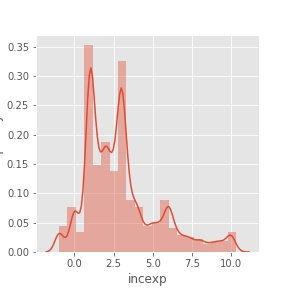
\includegraphics[width=\textwidth]{figures/hist_incexp}
		\end{subfigure}
		\begin{subfigure}[b]{0.45\textwidth}
			\centering
			\caption{expected growth of real}
			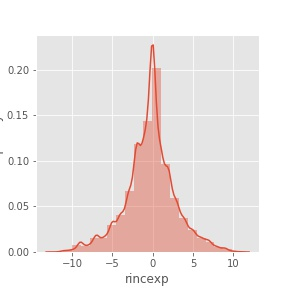
\includegraphics[width=\textwidth]{figures/hist_rincexp}
		\end{subfigure}
	\end{figure}
	\begin{itemize}
		\item nominal income: right-skewed and mostly positive   
		\item real income: symmetric around zero  
	\end{itemize}
\end{frame}

\begin{frame}{Cross-section of income risks}
	\begin{figure}
		\centering
		\label{incvar_hist}
			\begin{subfigure}[b]{0.45\textwidth}
			\centering
			\caption{nominal income risk}
		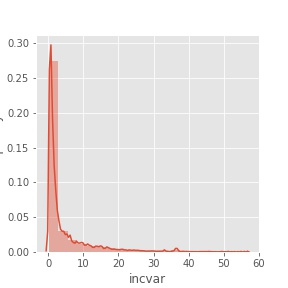
\includegraphics[width=\textwidth]{figures/hist_incvar}
		\end{subfigure}
		\begin{subfigure}[b]{0.45\textwidth}
		\centering
		\caption{real income risk}
		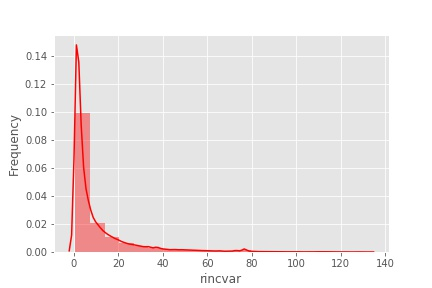
\includegraphics[width=\textwidth]{figures/hist_rincvar}
	\end{subfigure}
	\end{figure}
	\begin{itemize}
		\item average:  $2.5\%$ standard deviation for nominal and $3.5\%$ standard deviation for real income
		%\item just a lower bound: before adjustment of unemployment risk 
	\end{itemize}
\end{frame}

\begin{frame}{Cross-section of skewness (tail risks)}
	\begin{figure}
		\centering
		\label{incskew_hist}
		\begin{subfigure}[b]{0.45\textwidth}
			\centering
			\caption{nominal income skewness}
			\includegraphics[width=\textwidth]{figures/histincSkew}
		\end{subfigure}
	\end{figure}
	\begin{itemize}
		\item sizable dispersion in skewness, i.e. about half of the people has non-zero skewness in perceived income distribution. 
	\end{itemize}
\end{frame}



%\begin{frame}{Perceived income risks by household income}
%	\begin{figure}[ht]
%		\label{ts_incvar_HHinc_g_mean}
%		\begin{subfigure}[b]{0.7\textwidth}
%			\centering
%			\caption{income risks}
%			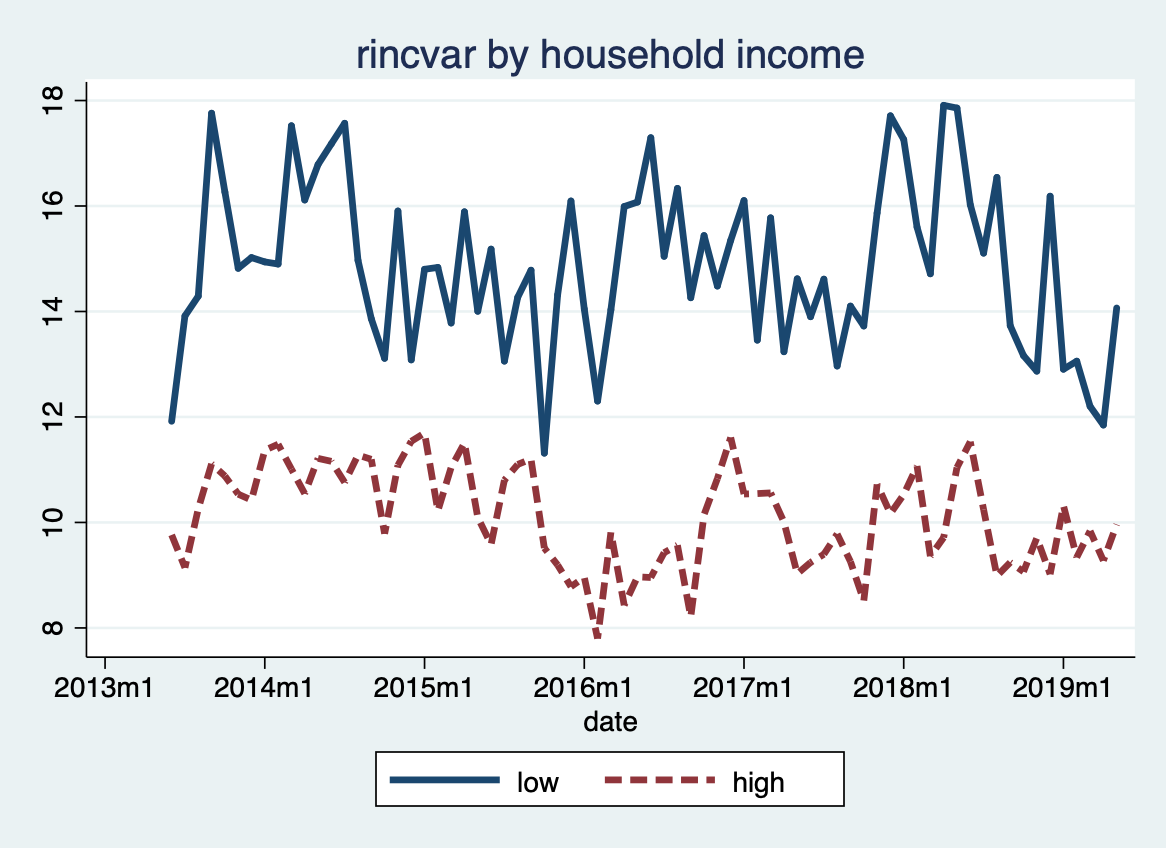
\includegraphics[width=\textwidth, height = 0.33\textheight]{figures/ts_rincvar_HHinc_g_mean.png}
%		\end{subfigure}
%		\begin{subfigure}[b]{0.7\textwidth}
%			\caption{skewness}
%			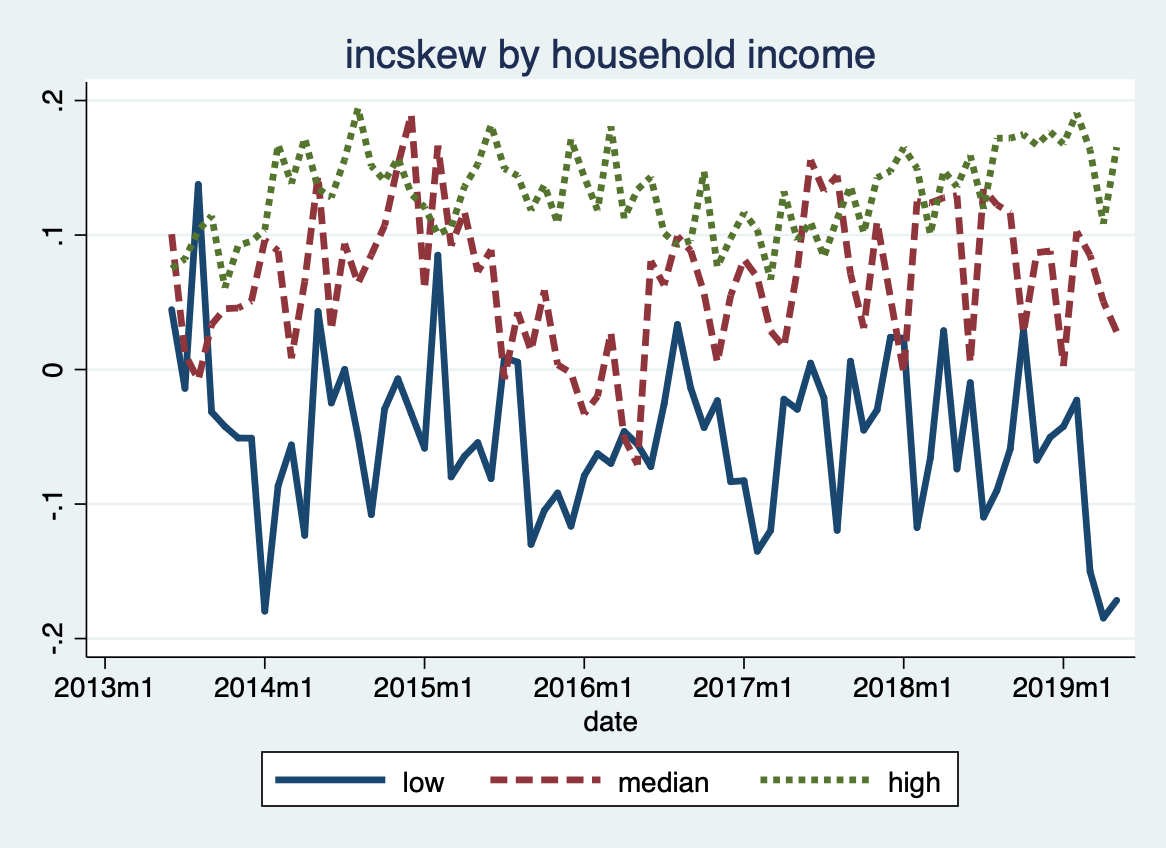
\includegraphics[width=\textwidth, height = 0.33\textheight]{figures/ts_incskew_HHinc_g_mean.png}
%		\end{subfigure}
%	\end{figure}
%\end{frame}


\begin{frame}{Perceived risks by household income}
\begin{figure}
	\centering
	\label{boxplot_hhinc}
	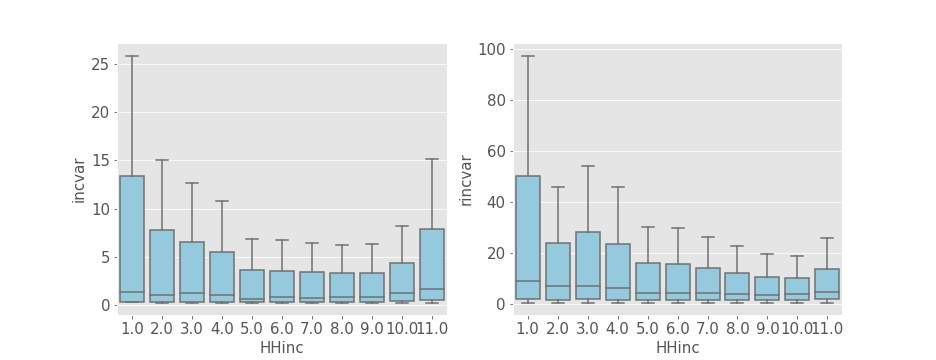
\includegraphics[width=0.8\textwidth]{figures/boxplot_var_HHinc}
\end{figure}
	\begin{itemize}
	\item Similar to the pattern of earning growth dispersion conditional on income in \cite{bloom2018great}. 
\end{itemize}
\end{frame}



\begin{frame}{Perceived risks by age}
	\begin{figure}[ht]
		\label{ts_incvar_age_g_mean}
		\begin{subfigure}[b]{0.46\textwidth}
			\centering
			\caption{risks}
			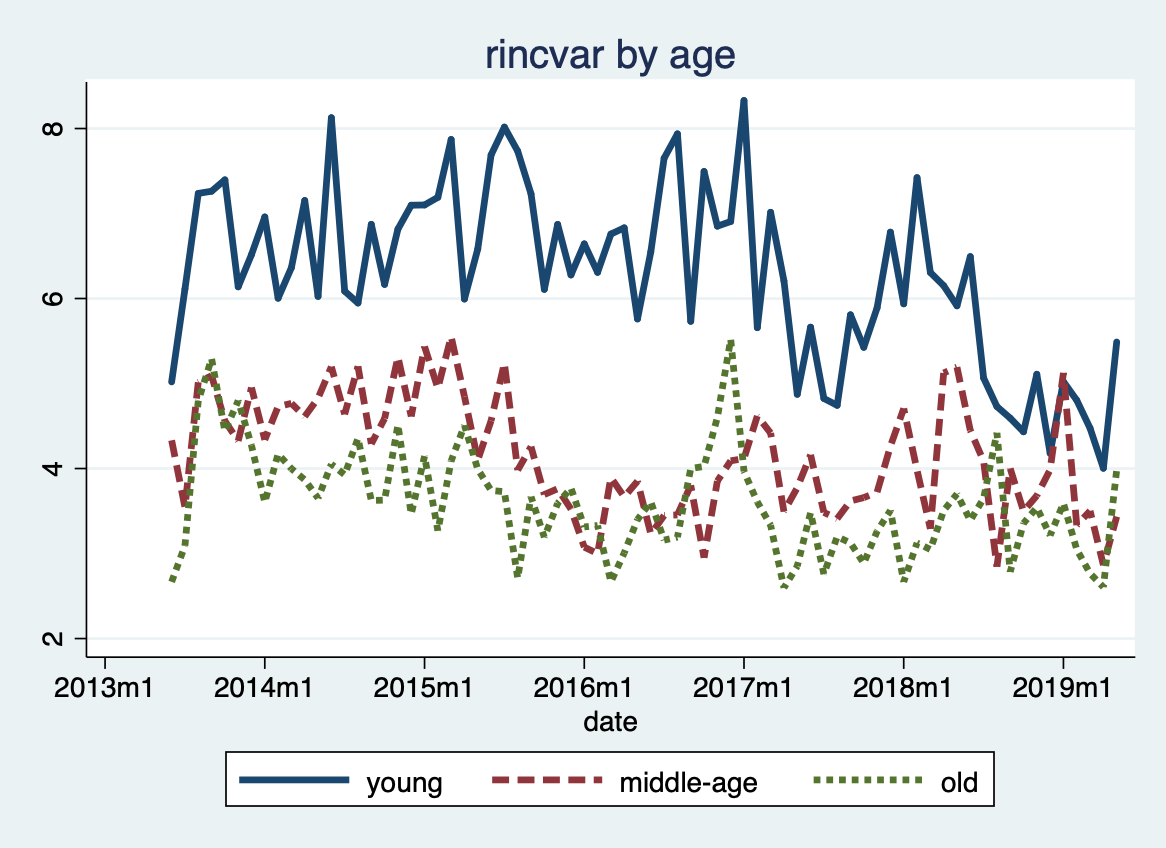
\includegraphics[width=\textwidth, height = 0.33\textheight]{figures/ts_rincvar_age_g_median.png}
		\end{subfigure}
		\begin{subfigure}[b]{0.46\textwidth}
			\caption{skewness}
			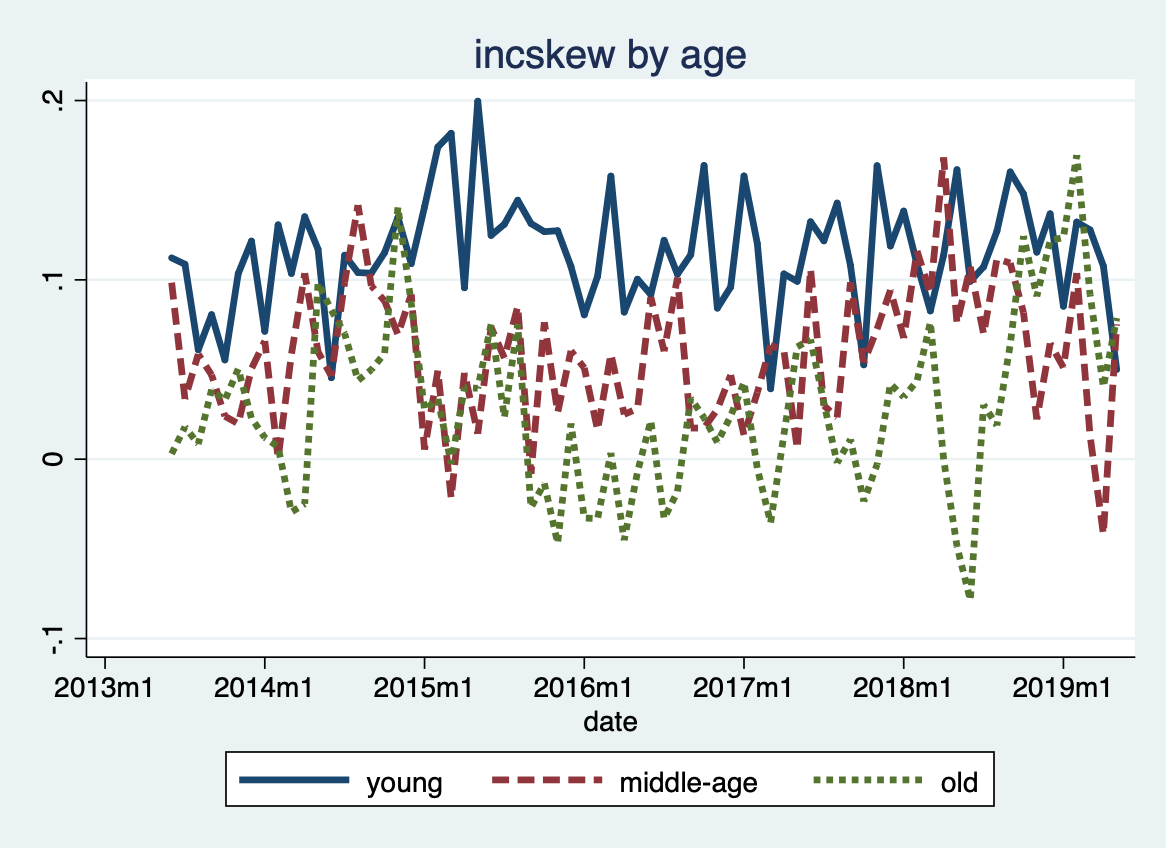
\includegraphics[width=\textwidth, height = 0.33\textheight]{figures/ts_incskew_age_g_mean.png}
	\end{subfigure}
	\end{figure}
\begin{itemize}
	\item in line with existing findings, for instance  
	\cite{bloom2018great}. 
\end{itemize}
 \end{frame}

%\begin{frame}{Perceived income risks by age}
%	\begin{figure}
%		\centering
%		\label{boxplot_age_gr}
%		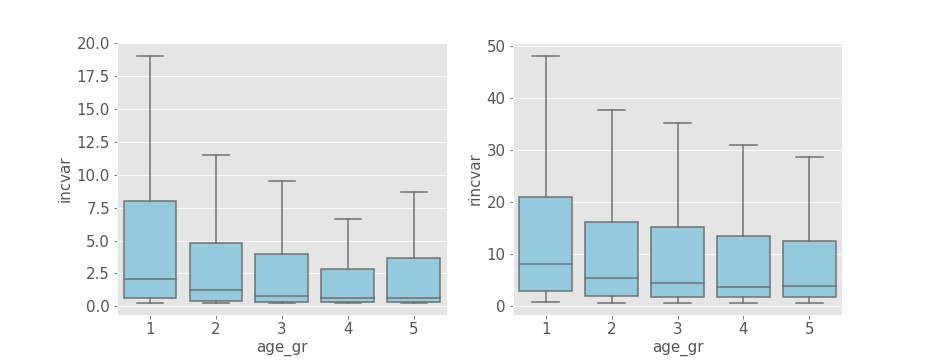
\includegraphics[width=0.8\textwidth]{figures/boxplot_exp_age_gr} \\
%		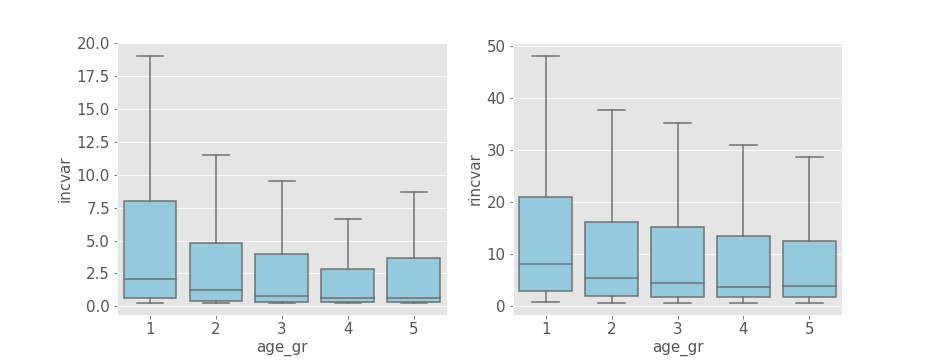
\includegraphics[width=0.8\textwidth]{figures/boxplot_var_age_gr}
%	\end{figure}
%	\begin{itemize}
%		\item 
%	\end{itemize}
%\end{frame}


\begin{frame}{Perceived risks by generation}
	\begin{figure}[ht]
		\label{ts_incvar_byear_g_mean}
		\begin{subfigure}[b]{0.46\textwidth}
			\centering
			\caption{risks}
			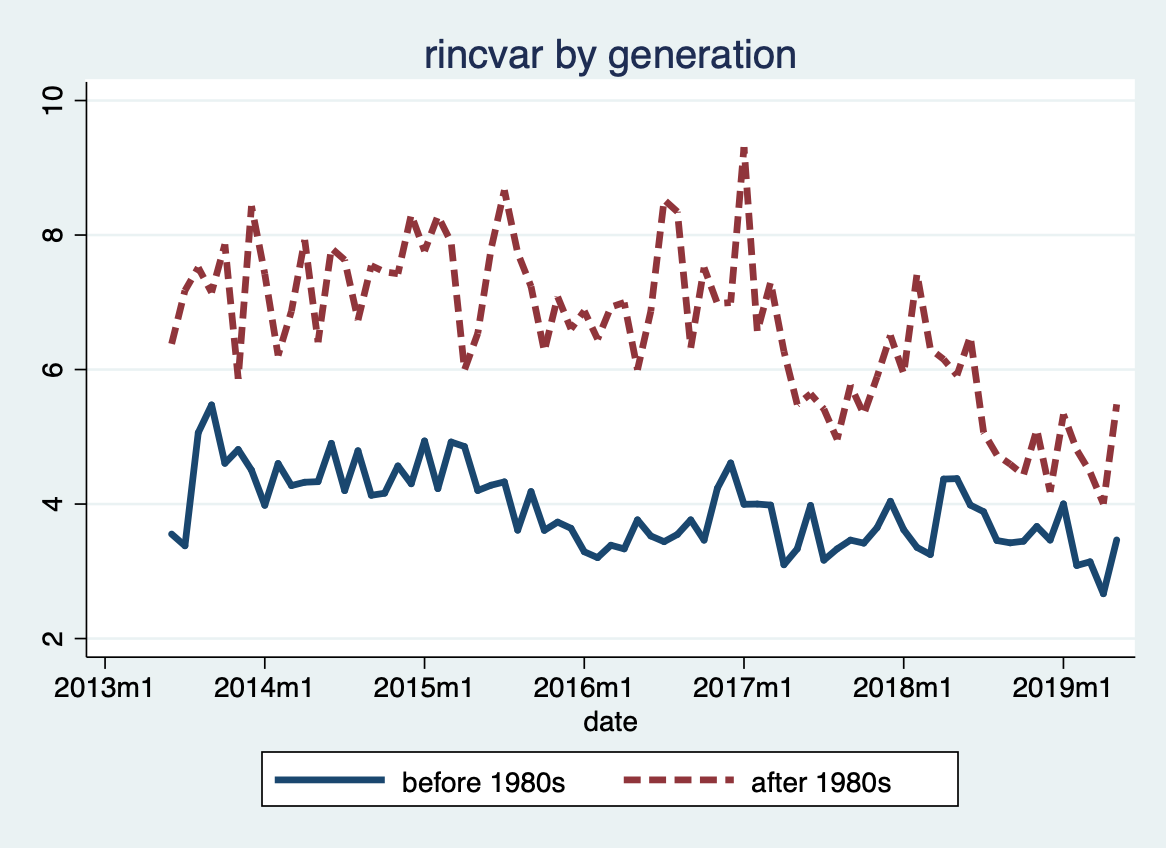
\includegraphics[width=\textwidth, height = 0.33\textheight]{figures/ts_rincvar_byear_g_median.png}
		\end{subfigure}
		\begin{subfigure}[b]{0.46\textwidth}
			\caption{skewness}
			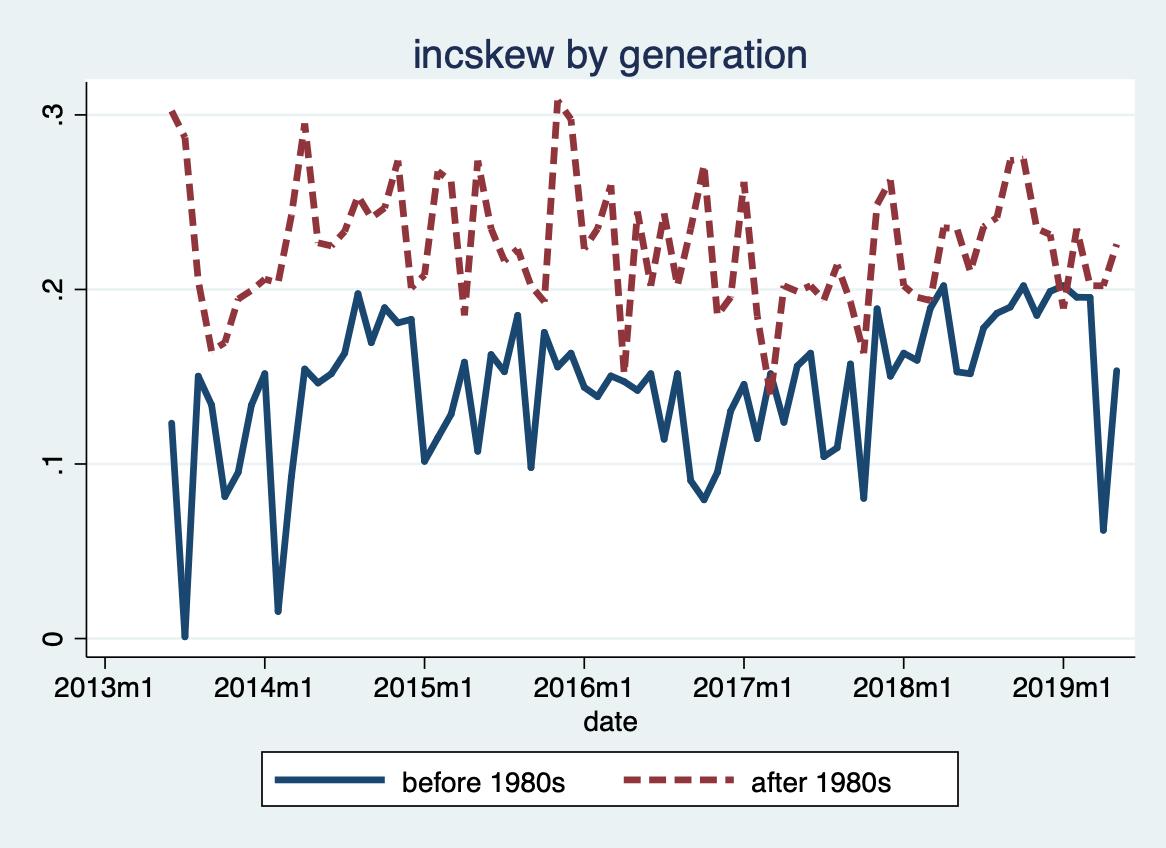
\includegraphics[width=\textwidth, height = 0.33\textheight]{figures/ts_incskew_byear_g_median.png}
		\end{subfigure}
	\end{figure}
\end{frame}


%\begin{frame}{Perceived income risks by generation}
%	\begin{figure}
%		\centering
	%	\label{boxplot_byear_gr}
%	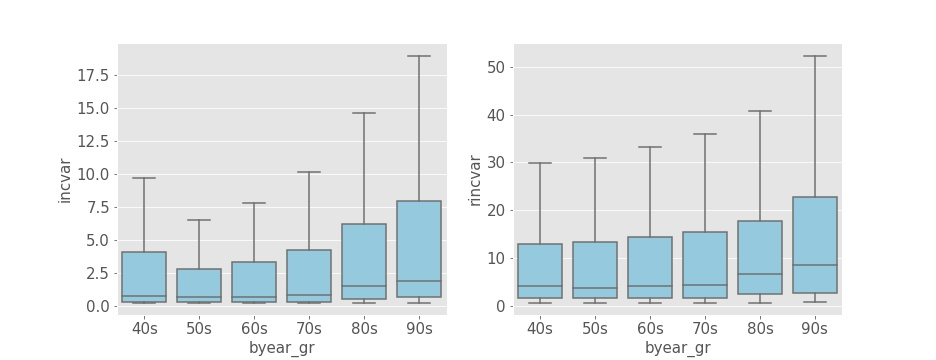
\includegraphics[width=0.8\textwidth]{figures/boxplot_var_byear_gr}
%	\end{figure}
%	\begin{itemize}
	%	\item 
%	\5end{itemize}
%\end{frame}


\begin{frame}{Perceived risks by education}
	\begin{figure}[ht]
		\label{ts_incvar_educ_g_mean}
		\begin{subfigure}[b]{0.46\textwidth}
			\centering
			\caption{risks}
			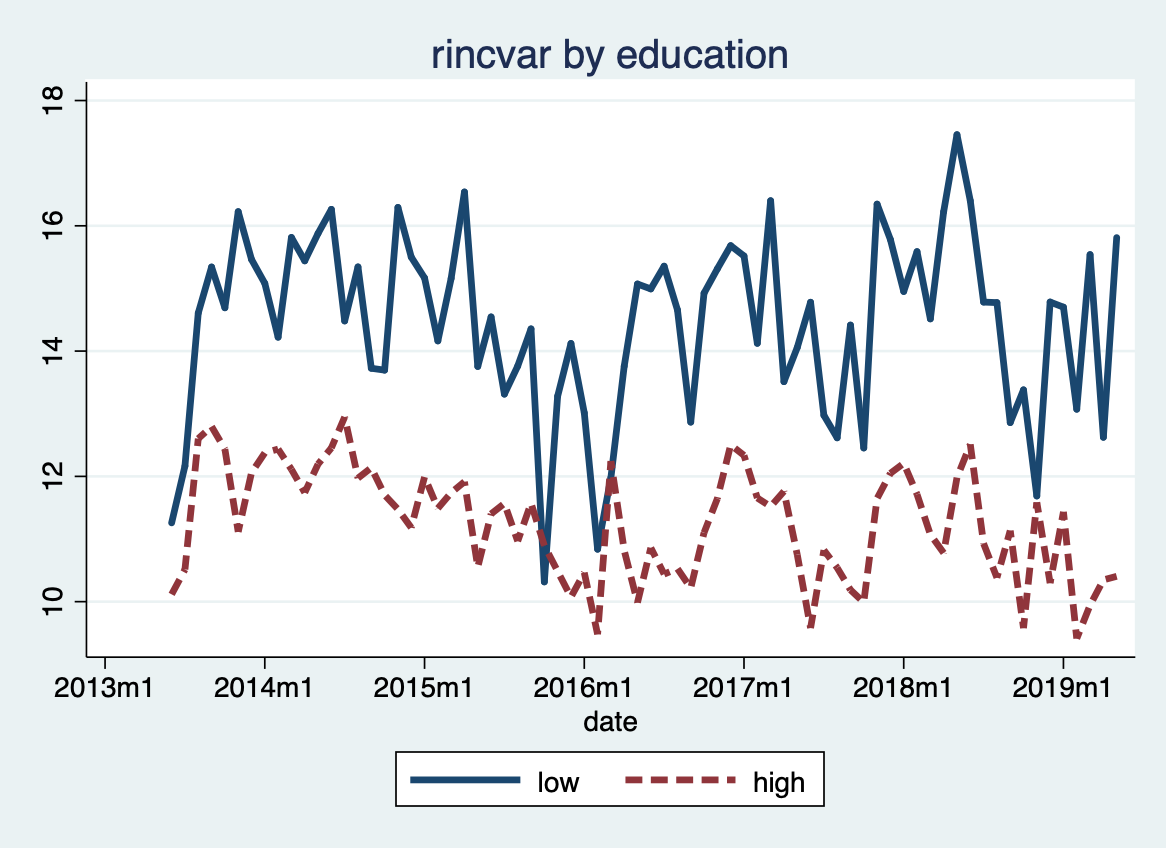
\includegraphics[width=\textwidth, height = 0.33\textheight]{figures/ts_rincvar_edu_g_mean.png}
		\end{subfigure}
		\begin{subfigure}[b]{0.46\textwidth}
			\caption{skewness}
			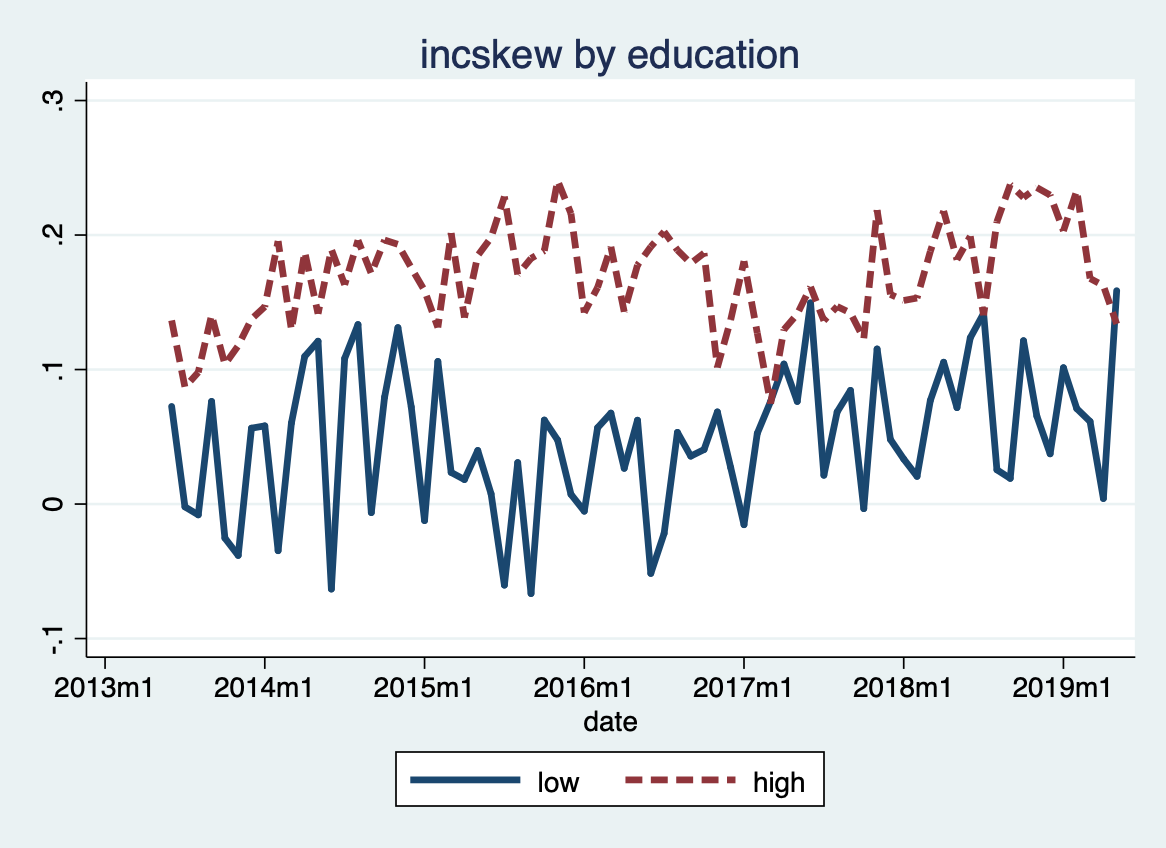
\includegraphics[width=\textwidth, height = 0.33\textheight]{figures/ts_incskew_edu_g_mean.png}
		\end{subfigure}
	\end{figure}
	\begin{itemize}
			\item not the same to some other findings, for instance  
			\cite{meghir2004income}
		\end{itemize}
\end{frame}


%\begin{frame}{Perceived income risks by education}
%	\begin{figure}
%		\centering
%		\label{boxplot_educ_gr}
%		\includegraphics[width=0.8\textwidth]{figures/boxplot_exp_edu_gr} \\
%		\includegraphics[width=0.8\textwidth]{figures/boxplot_var_edu_gr}
%	\end{figure}
%	\begin{itemize}
%		\item 
%	\end{itemize}
% \end{frame}



\begin{frame}{Covariants of perceived risks}
	\begin{table}
		\centering
		\caption{Perceived income risks and individual characteristics}
		\label{micro_reg}
		\adjustbox{max height=0.5\textheight, max width=\textwidth}{ 
\begin{tabular}{ccccccccc}
	\hline 
	{} & incvar I & incvar II & incvar III & incvar IIII & rincvar I & rincvar II & rincvar III & rincvar IIII \\
	\hline 
	HHinc\_gr=low inc &          &           &    1.56*** &             &           &            &     7.01*** &              \\
	&          &           &     (0.10) &             &           &            &      (0.19) &              \\
	educ\_gr=low educ &          &           &            &     0.40*** &           &            &             &      3.82*** \\
	&          &           &            &      (0.11) &           &            &             &       (0.21) \\
	gender=male      &          &           &            &    -0.80*** &           &            &             &      2.76*** \\
	&          &           &            &      (0.10) &           &            &             &       (0.19) \\
	parttime=yes     &     0.05 &     0.24* &      -0.12 &             &   1.41*** &    1.81*** &        0.19 &              \\
	&   (0.12) &    (0.13) &     (0.13) &             &    (0.23) &     (0.26) &      (0.26) &              \\
	selfemp=yes      &  7.21*** &  -0.00*** &   -0.00*** &             &   6.27*** &   -0.00*** &     0.00*** &              \\
	&   (0.15) &    (0.00) &     (0.00) &             &    (0.27) &     (0.00) &      (0.00) &              \\
	UEprobAgg        &          &    0.01** &      0.00* &             &           &    0.05*** &     0.04*** &              \\
	&          &    (0.00) &     (0.00) &             &           &     (0.00) &      (0.00) &              \\
	UEprobInd        &          &   0.03*** &    0.02*** &             &           &    0.05*** &     0.04*** &              \\
	&          &    (0.00) &     (0.00) &             &           &     (0.00) &      (0.00) &              \\
	Intercept        &  4.64*** &   3.75*** &    3.28*** &     5.72*** &  12.42*** &   12.21*** &    10.16*** &     11.16*** \\
	&   (0.05) &    (0.12) &     (0.12) &      (0.07) &    (0.10) &     (0.24) &      (0.25) &       (0.14) \\
	\hline 
	N                &    54029 &     47331 &      47331 &       47457 &     50730 &      44382 &       44382 &        44517 \\
	R2               &     0.05 &      0.00 &       0.01 &        0.00 &      0.01 &       0.01 &        0.04 &         0.01 \\
	\hline 
\end{tabular}
}
	\end{table}
\end{frame}


\subsection{Perceived risks and decisions}


\begin{frame}{Perveived risks and household spending}
	
\begin{eqnarray*}
	E_{i,t} (\Delta C_{i,t+12}) = u_0 + u_1 \overline{\text{risks}}_{i,t} (\Delta Y_{i,t+12}) + \xi_{i,t}  
\end{eqnarray*}
	\begin{table}
		\centering
		%\caption{Perceived income risks and household spending}
		\label{spending_reg}
		\adjustbox{max height=0.5\textheight, max width=\textwidth}{ 
	
	\begin{tabular}{ccccccll}
		\hline 
		{} & spending I & spending II & spending III & spending IIII & spending IIIII & spending IIIIII & spending IIIIIII \\
		\hline 
		incexp    &    0.39*** &             &              &               &                &                 &                  \\
		&     (0.08) &             &              &               &                &                 &                  \\
		
		rincexp   &            &      -0.04* &              &               &                &                 &                  \\
		&            &      (0.02) &              &               &                &                 &                  \\
		incvar    &            &             &      0.07*** &               &                &                 &                  \\
		&            &             &       (0.02) &               &                &                 &                  \\
		
		rincvar   &            &             &              &       0.07*** &                &                 &                  \\
		&            &             &              &        (0.01) &                &                 &                  \\
		
		UEprobAgg &            &             &              &               &                &         0.04*** &                  \\
		&            &             &              &               &                &          (0.01) &                  \\
		UEprobInd &            &             &              &               &          -0.01 &                 &                  \\
		&            &             &              &               &         (0.01) &                 &                  \\
		
		incskew   &            &             &              &               &                &                 &             0.21 \\
		&            &             &              &               &                &                 &           (0.43) \\
		\hline 
		N         &      55673 &       50997 &        55465 &         52099 &          54315 &           85468 &            55029 \\
		R2        &       0.00 &        0.00 &         0.00 &          0.00 &           0.00 &            0.00 &             0.00 \\
		\hline 
	\end{tabular}
		}
	\end{table}
\begin{itemize}
	\item  Higher perceived risks $\rightarrow$ higher expected spending growth. 
\end{itemize}
\end{frame}


\subsection{Correlation with the stock market}


\begin{frame}{Perceived risks and \textcolor{red}{expected} stock performance}
	
	\begin{eqnarray*}
		\overline{\text{risk}_{i,t}}= a_0 + a_1 \underbrace{Stkprob_{i,t}}_{\text{probability of stock market goes up next year }} + \eta_{i,t}
	\end{eqnarray*}
	
	\begin{table}
		\centering
		%\caption{Correlation between Perceived Income Risks and Stock Market Return}
		\label{macro_corr_stk_ind}
		\adjustbox{max height=0.5\textheight, max width=\textwidth}{ 
			\begin{tabular}{lllll}
				\hline 
				& incvar   & rincvar   & inciqr   & incskew  \\
				\hline 
				Stkprob & 0.014*** & -0.018*** & 0.005*** & 0.001*** \\
				& (0.002)  & (0.004)   & (0.000)  & (0.000)  \\
				&          &           &          &          \\
				Constant   & 2.793*** & 9.616***  & 1.821*** & 0.078*** \\
				& (0.087)  & (0.178)   & (0.022)  & (0.005)  \\
				&          &           &          &          \\
				\hline 
				N       & 30121    & 30121     & 30121    & 30121    \\
				r2      & 0.002    & 0.001     & 0.005    & 0.002   \\
				\hline 
			\end{tabular}
		}
	\end{table}
\end{frame}


\begin{frame}{Perceived risks and stock market performance}
	\begin{itemize}
		\item $\overline{\text{var}_{t}} $
\item  $log(\text{sp500}_{t+12}) - log(\text{sp500}_{t})$
\end{itemize}
	\begin{figure}
		\centering
		\label{ts_var}
		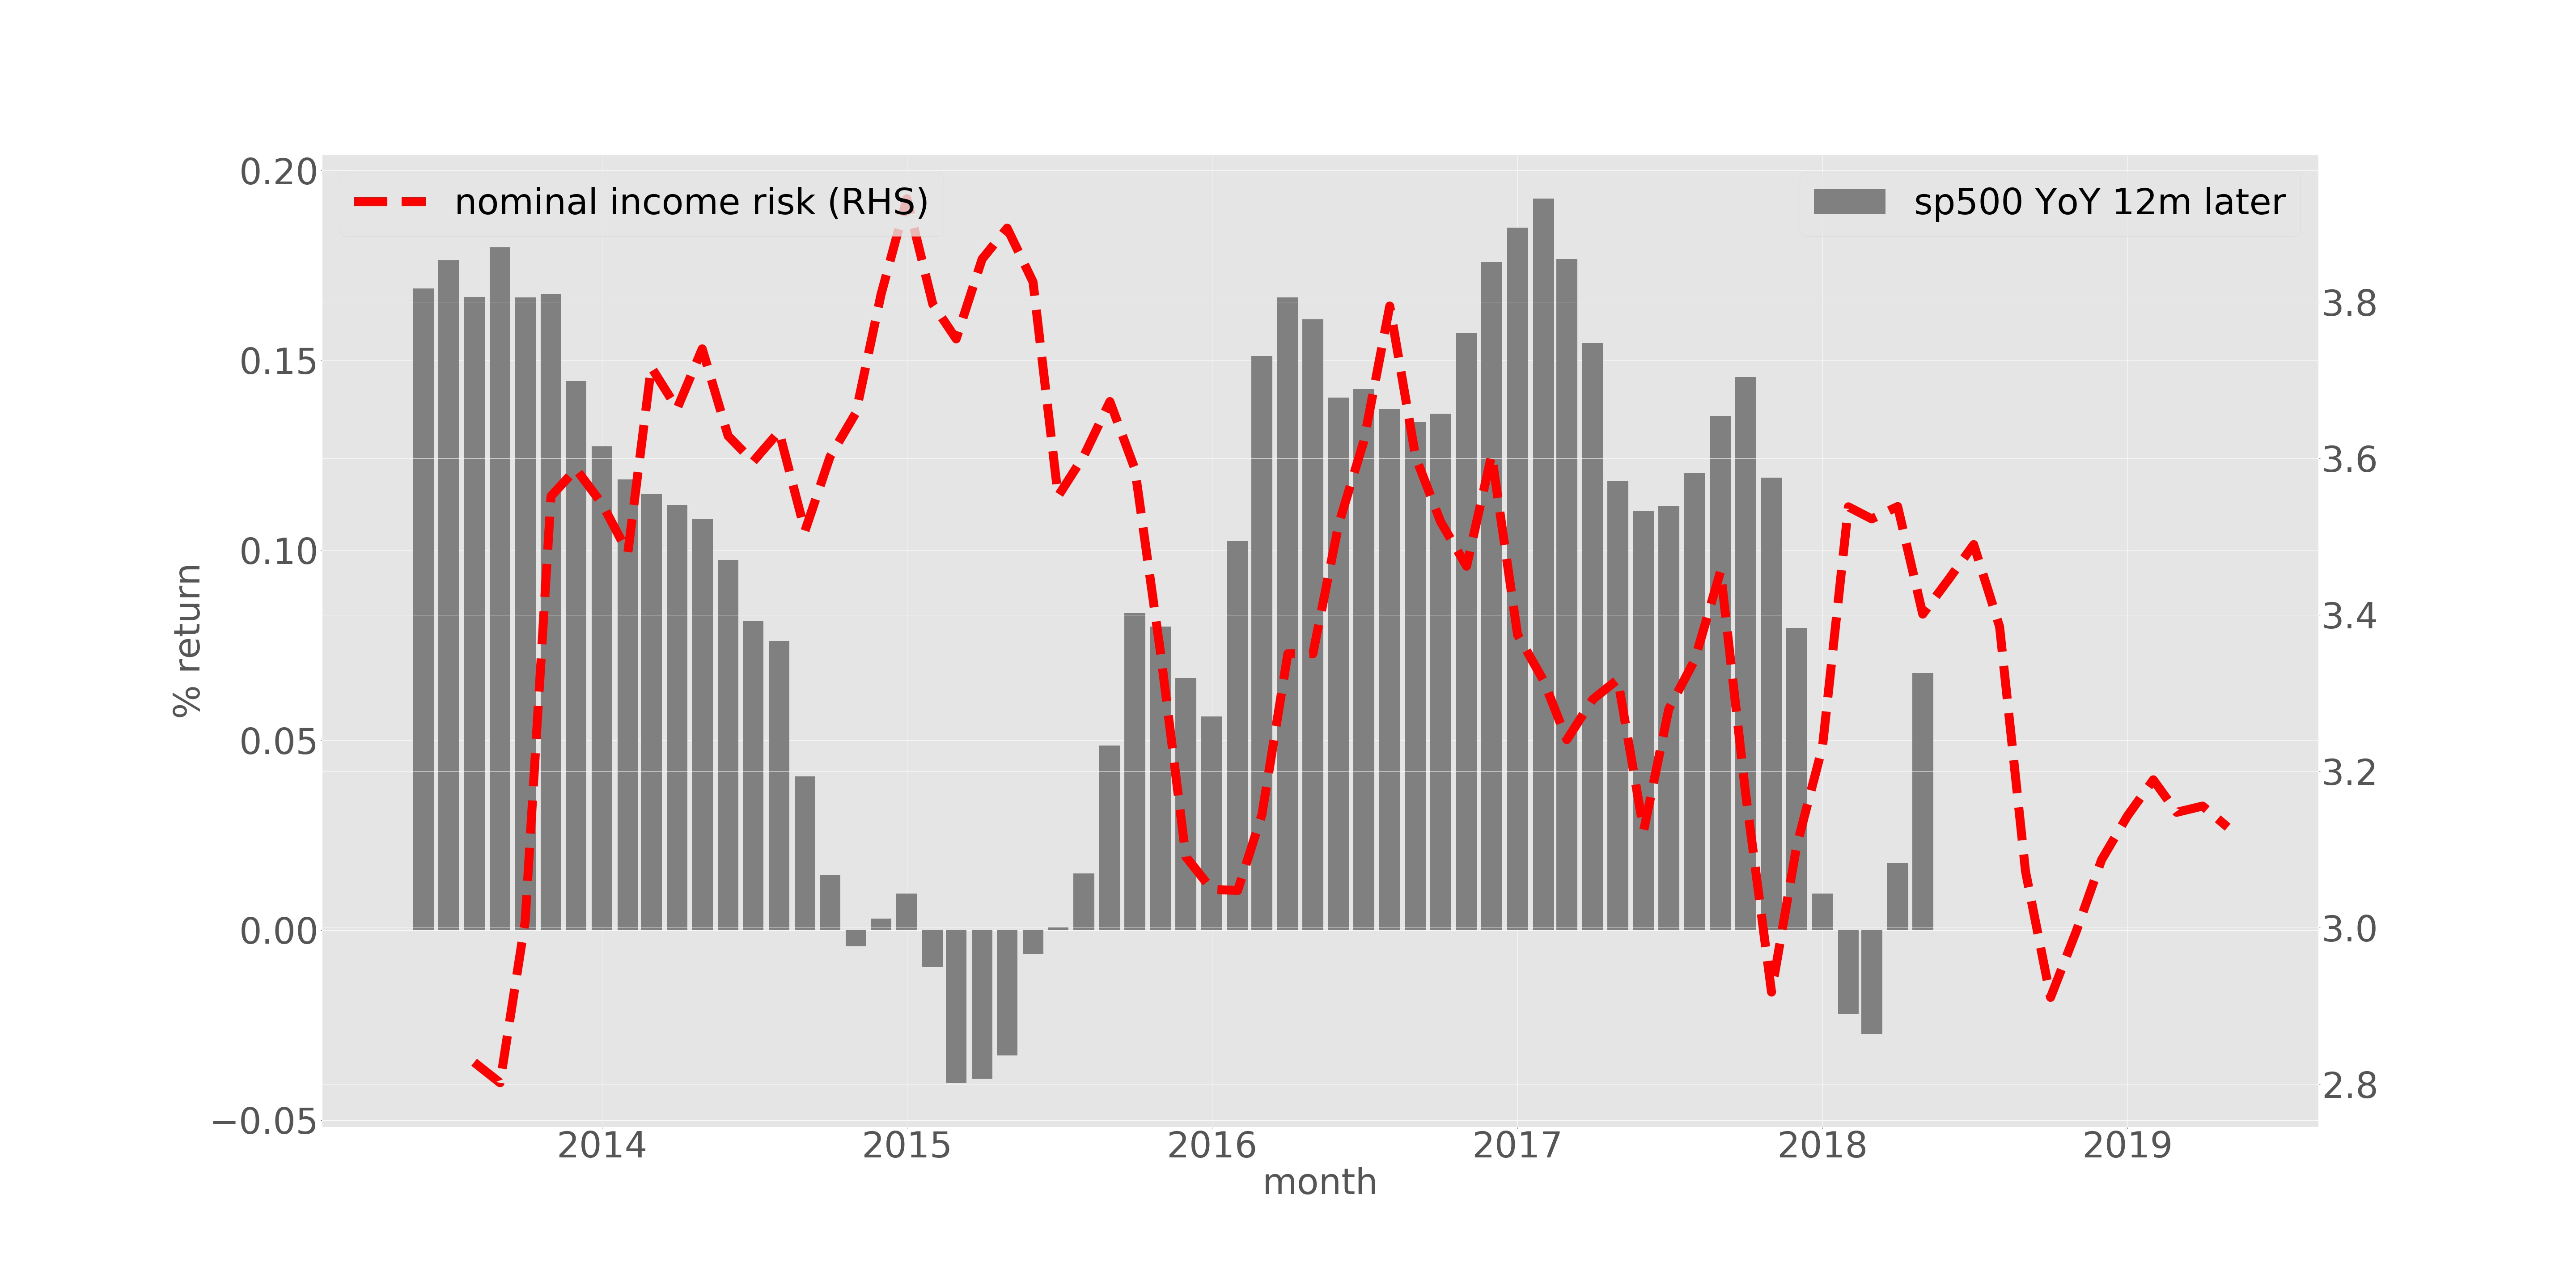
\includegraphics[width=\textwidth]{figures/tsMean3mvvar.jpg}
	\end{figure}
\end{frame}


\begin{frame}{Perceived skewness and stock market performance}
	\begin{itemize}
	\item $\overline{\text{skew}_{t}} $
	\item  $log(\text{sp500}_{t+12}) - log(\text{sp500}_{t})$
\end{itemize}
	\begin{figure}
		\centering 
		\label{ts_skew}
		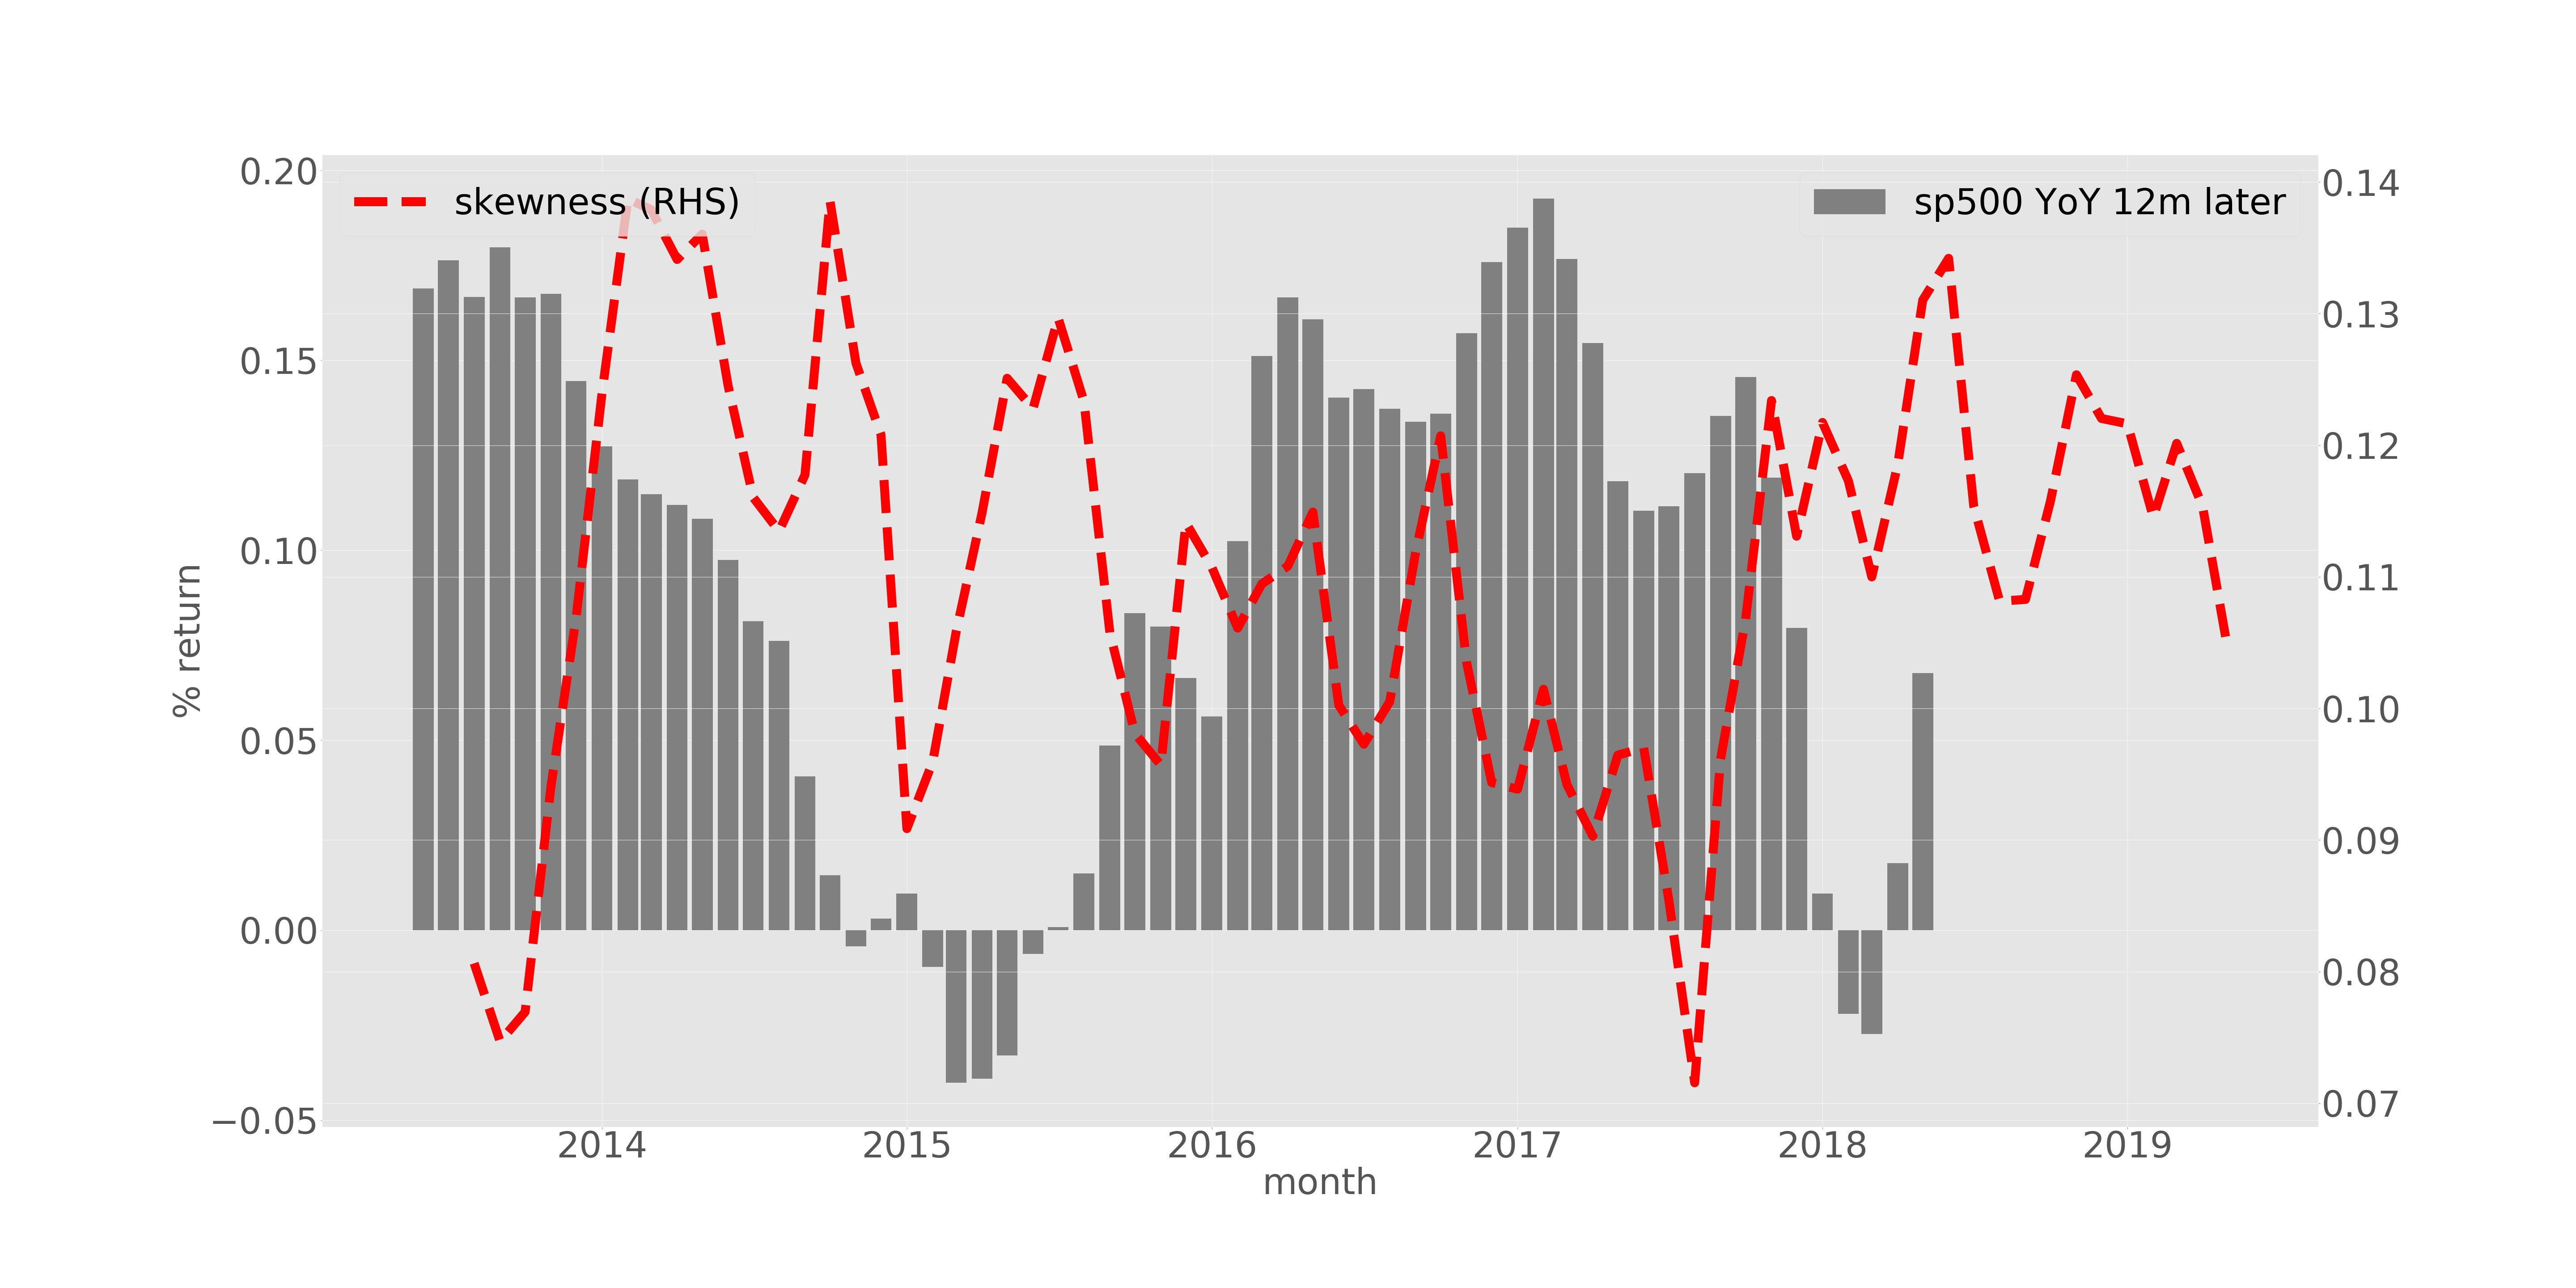
\includegraphics[width=\textwidth]{figures/tsMean3mvskew.jpg}
	\end{figure}
\end{frame}


\begin{frame}{Perceived risks and stock market performance}
	
	\begin{eqnarray*}
\underbrace{\overline{\text{risk}_{t}}}_{\text{average perceived risk}} = \alpha + \textcolor{red}{\beta} \underbrace{(log(\text{sp500}_{t+k}) - log(\text{sp500}_{t+k-12}))}  _{\text{stock market return}}  + \epsilon_{i,t}	\\
\quad \forall k =1...12
	\end{eqnarray*}

\begin{table}
	\centering
%\caption{Correlation between Perceived Income Risks and Stock Market Return}
\label{macro_corr}
	\adjustbox{max height=0.5\textheight, max width=\textwidth}{ \begin{tabular}{lllllllll}
				\hline 
			\# months ahead & varMean   & iqrMean   & rvarMean & skewMean  & varMed & iqrMed & rvarMed & skewMed \\
				\hline 
			1              & 0.229     & 0.146     & 1.509    & 0.023     & -0.061 & -0.014 & 0.457   & NA      \\
			2              & 0.517     & 0.199     & 2.457    & -0.009    & -0.13  & -0.065 & 0.74    & NA      \\
			3              & 0.469     & 0.194     & 3.784**  & -0.052*   & -0.119 & -0.061 & 0.695   & NA      \\
			4              & 0.17      & 0.112     & 3.098    & -0.051    & -0.116 & -0.052 & 0.358   & NA      \\
			5              & -0.472    & -0.07     & 0.701    & -0.028    & -0.126 & -0.027 & -0.117  & NA      \\
			6              & -0.275    & -0.056    & 0.057    & -0.018    & -0.229 & -0.122 & -0.709  & NA      \\
			7              & -0.63     & -0.164    & -0.158   & -0.049    & -0.195 & -0.115 & -0.959  & NA      \\
			8              & -1.048**  & -0.298*   & -1.827   & -0.076*   & -0.279 & -0.181 & -1.655* & NA      \\
			9              & -1.239*** & -0.368**  & -1.886   & -0.065**  & -0.25  & -0.173 & -1.689* & NA      \\
			10             & -1.727*** & -0.513*** & -2.597*  & -0.061**  & -0.258 & -0.163 & -1.489  & NA      \\
			11             & -2.038*** & -0.567*** & -2.41*   & -0.089*** & -0.201 & -0.113 & -1.568* & NA      \\
			12             & -1.416*** & -0.467*** & -1.543   & -0.088*** & -0.267 & -0.179 & -1.37   & NA    \\
			\hline  
		\end{tabular}
}
\end{table}

\begin{itemize}
	\item Newey-west s.e.and bias correction \cite{stambaugh_predictive_1999}. 
\end{itemize}	

\end{frame}


\begin{frame}{Perceived risks and stock market performance}
	\begin{figure}
		\centering
		\label{corr_stk}
		\begin{subfigure}[b]{0.45\textwidth}
			\centering
			\caption{variance and \textcolor{red}{yearly} return}
			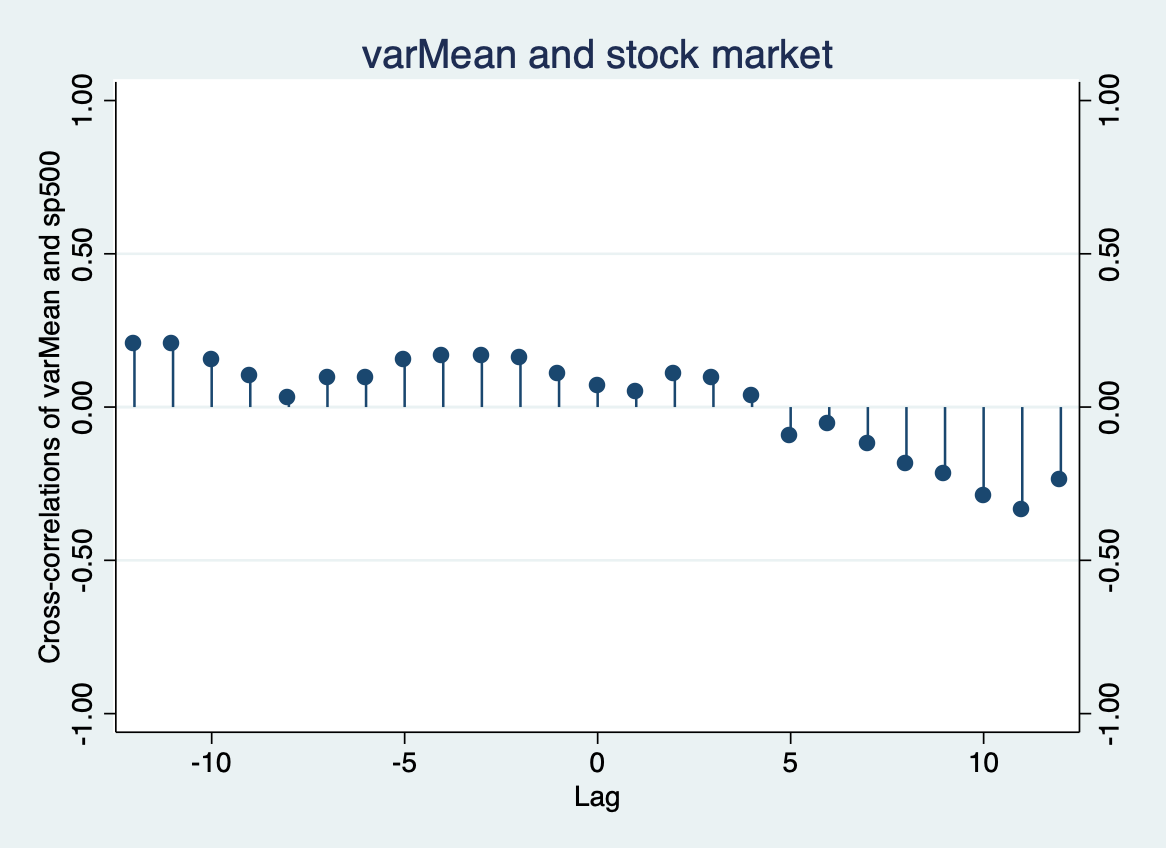
\includegraphics[width=\textwidth]{figures/corr_varMean_stk}
		\end{subfigure}
		\begin{subfigure}[b]{0.45\textwidth}
			\centering
			\caption{skewness and \textcolor{red}{yearly} return}
			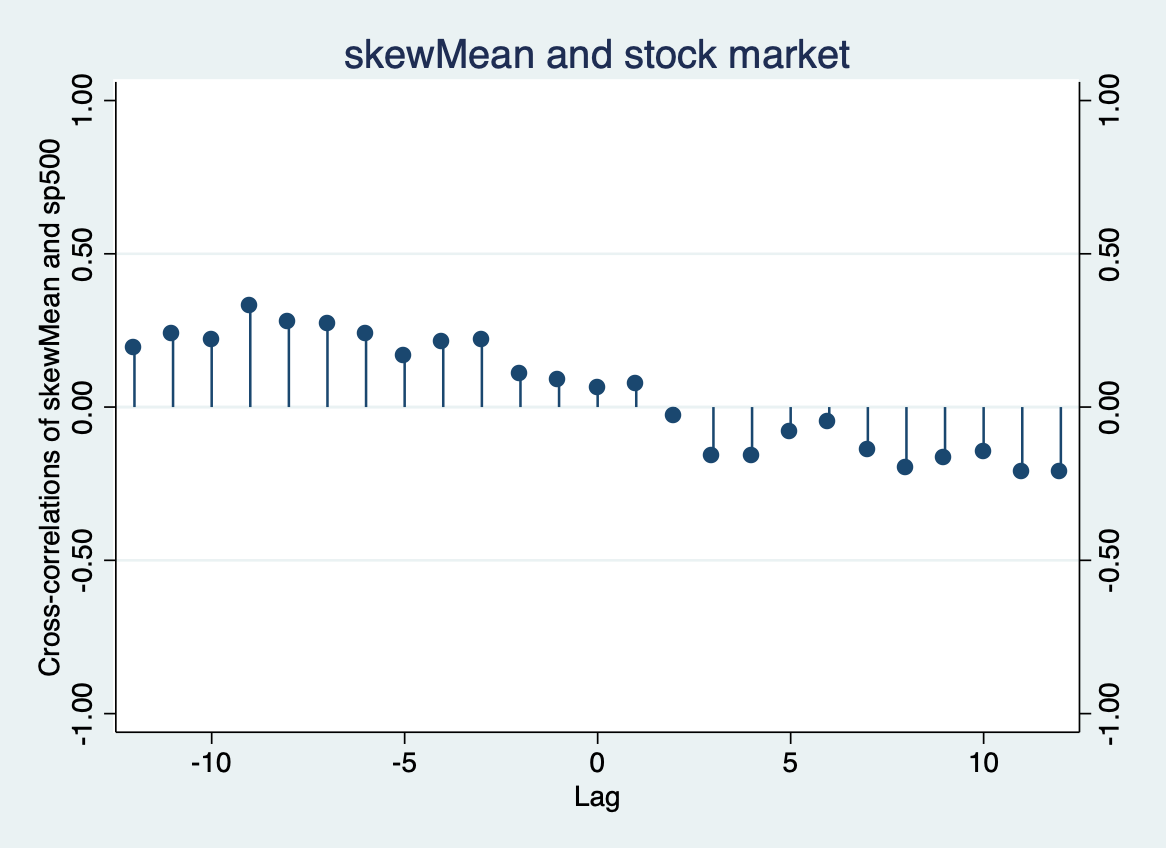
\includegraphics[width=\textwidth]{figures/corr_skewMean_stk}
		\end{subfigure}
	\end{figure}
\end{frame}


\begin{frame}{Perceived risks and stock market performance}
	
	\begin{eqnarray*}
		\underbrace{\overline{\text{risk}_{t}}}_{\text{average perceived risk}} = \alpha + \textcolor{red}{\beta} \underbrace{(log(\text{sp500}_{t+k}) - log(\text{sp500}_{t+k-1}))}  _{\text{stock market return}}  + \epsilon_{i,t}	\\
		\quad \forall k =1...12
	\end{eqnarray*}
	

	\begin{table}
		\centering
		%\caption{Correlation between Perceived Income Risks and Stock Market Return}
		\label{macro_corr_monthly}
		\adjustbox{max height=0.5\textheight, max width=\textwidth}{ 
			\begin{tabular}{lllllllll}
				\hline 
				\# months ahead & varMean & iqrMean & rvarMean & skewMean & varMed & iqrMed & rvarMed & skewMed \\
				\hline 
				1              & -0.387  & -0.129  & 0.711    & 0.065    & -0.341 & -0.27  & 0.161   & NA      \\
				2              & 0.423   & 0.102   & 3.056    & -0.178** & -0.204 & -0.176 & 1.081   & NA      \\
				3              & -0.299  & -0.124  & 4.03     & -0.007   & -0.261 & -0.162 & -0.886  & NA      \\
				4              & -1.405  & -0.397  & -1.763   & -0.053   & -0.084 & 0.026  & -0.979  & NA      \\
				5              & -2.249  & -0.55   & -8.515** & 0.079    & 0.15   & 0.218  & -0.723  & NA      \\
				6              & 0.218   & 0.009   & -1.339   & -0.015   & -0.304 & -0.308 & -2.202  & NA      \\
				7              & -0.95   & -0.433  & -0.738   & -0.174*  & -0.236 & -0.182 & -2.189  & NA      \\
				8              & -1.36   & -0.431  & -4.698   & -0.01    & -0.202 & -0.169 & -2.138  & NA      \\
				9              & -0.889  & -0.199  & -1.114   & 0.021    & 0.105  & 0.069  & 0.256   & NA      \\
				10             & -2.347  & -0.597  & -2.284   & 0.02     & 0.163  & 0.162  & 0.927   & NA      \\
				11             & -1.641  & -0.398  & -1.282   & -0.126   & 0.103  & 0.06   & -1.841  & NA      \\
				12             & 3.55**  & 0.708*  & 5.111    & -0.016   & -0.22  & -0.144 & 1.21    & NA     \\
				\hline
			\end{tabular}
		}
	\end{table}
\end{frame}


\begin{frame}{Perceived risks and stock market performance}
	
	\begin{figure}
		\centering
		\label{corr_stk_monthly}
		\begin{subfigure}[b]{0.45\textwidth}
			\centering
			\caption{variance and \textcolor{red}{monthly} return}
			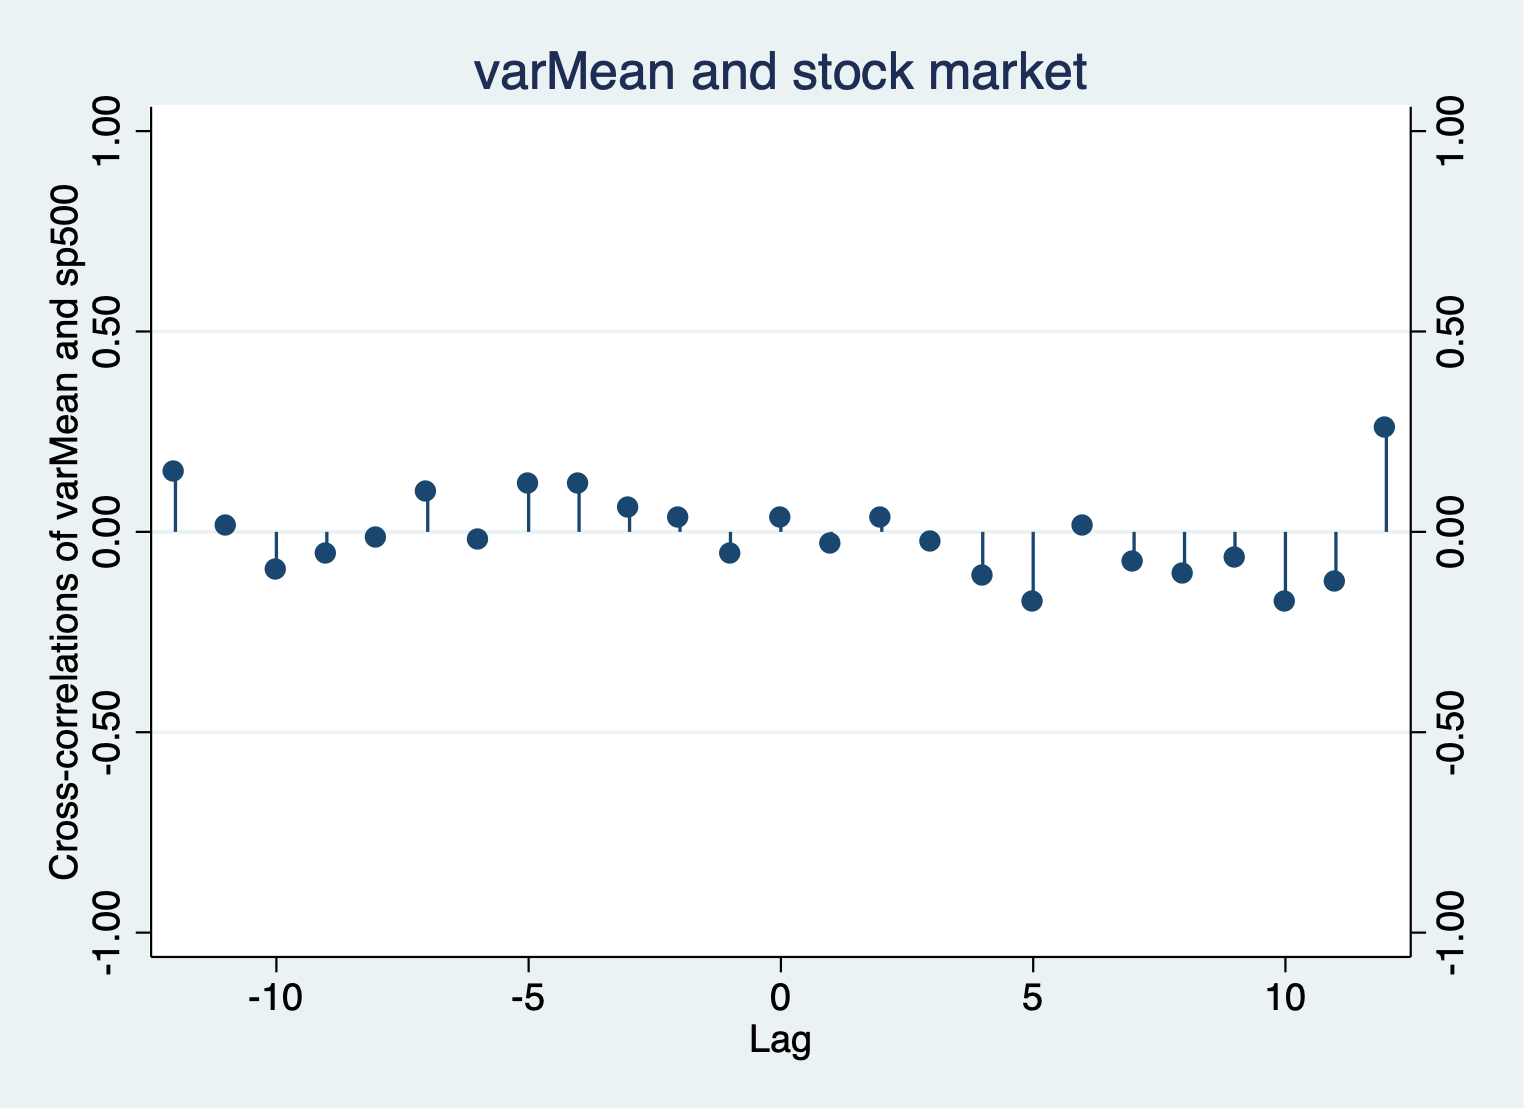
\includegraphics[width=\textwidth]{figures/corr_varMean_stk_monthly}
		\end{subfigure}
		\begin{subfigure}[b]{0.45\textwidth}
			\centering
			\caption{skewness and \textcolor{red}{monthly} return}
			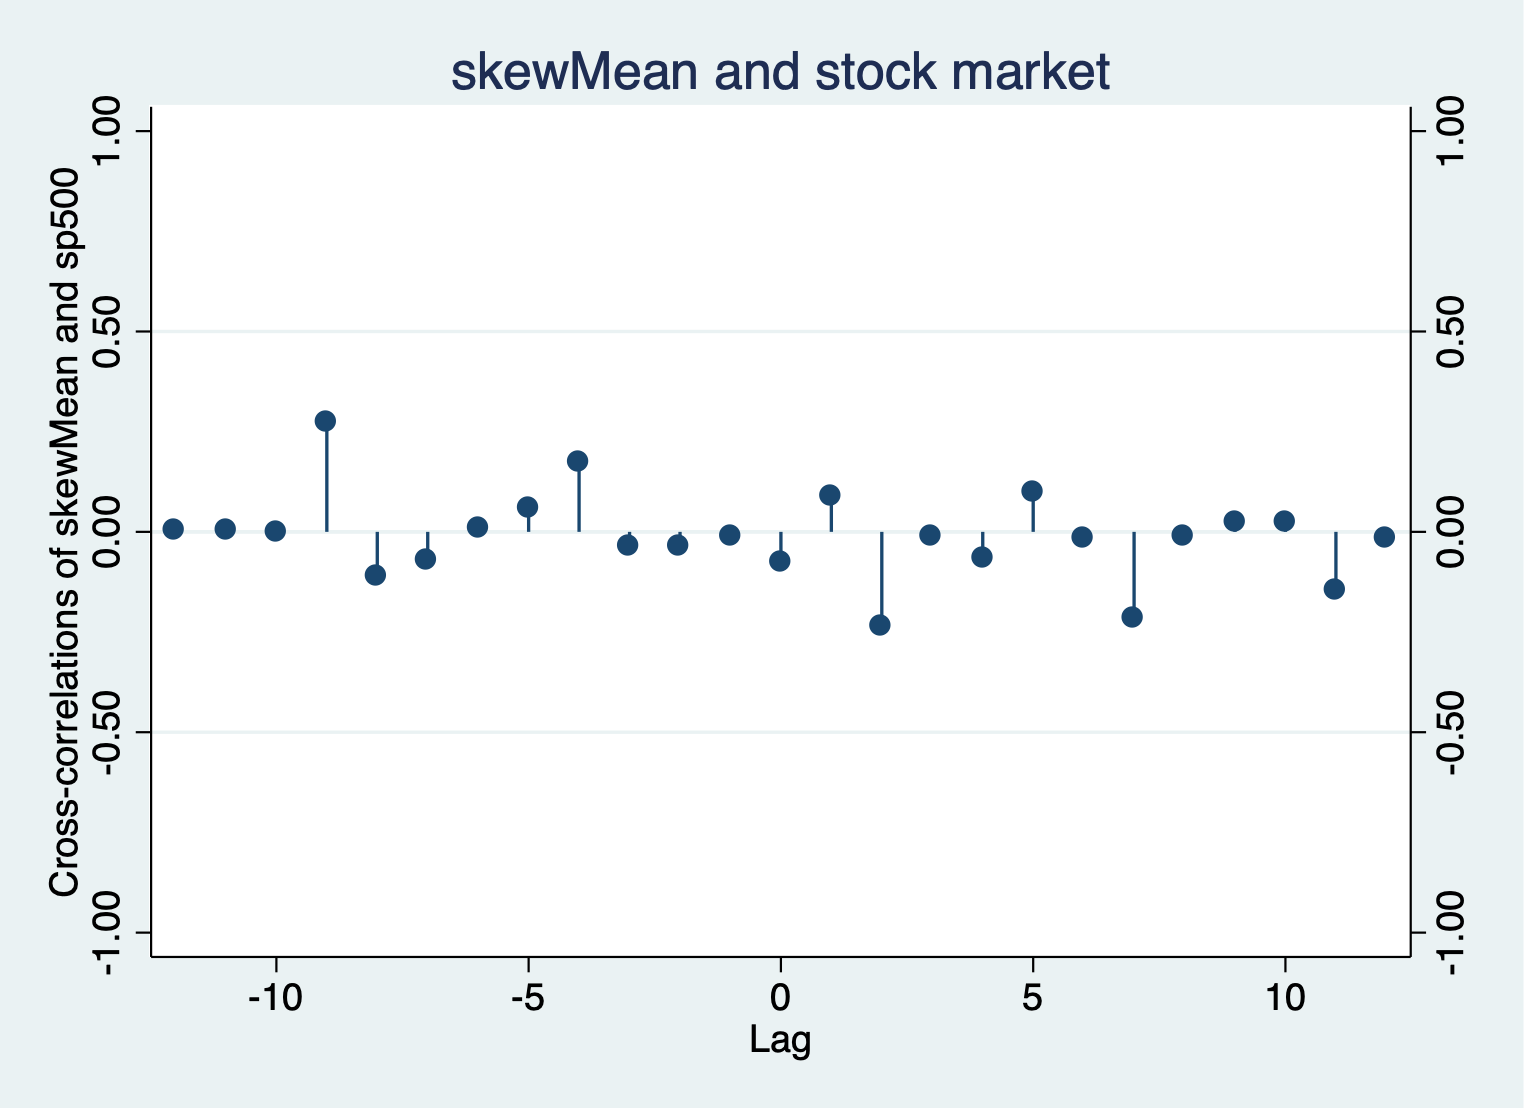
\includegraphics[width=\textwidth]{figures/corr_skewMean_stk_monthly}
		\end{subfigure}
	\end{figure}
\end{frame}




%\begin{frame}{Perceived income risks and stock market performance by income}
%	\begin{table}
%		\centering
%		\caption{Correlation between Perceived Income Risks and Stock Market Return}
%		\label{macro_corr_HHinc}
%		\adjustbox{max height=0.5\textheight, max width=\textwidth}{ 
%		\begin{tabular}{lllllllllllll}
%				\hline 
%			{leads} & 0                     & 1       & 2       & 3        & 4       & 5     & 6       & 7       & 8        & 9        & 10       & 11             \\
%			\hline 
%			mean:incvar for low   & 0.14    & 0.18    & 0.21*    & 0.25**  & 0.19  & 0.25**  & 0.23*   & 0.16     & 0.15     & 0.02     & -0.1    & -0.08   \\
%			mean:incvar for high  & 0.01    & 0.06    & 0.06     & -0.03   & -0.16 & -0.19   & -0.27** & -0.33*** & -0.39*** & -0.43*** & -0.4*** & -0.27** \\
%			mean:rincvar for low  & 0.09    & 0.16    & 0.23*    & 0.28**  & 0.1   & 0.17    & 0.16    & 0.08     & 0.15     & 0.05     & -0.0    & 0.08    \\
%			mean:rincvar for high & 0.13    & 0.2     & 0.26**   & 0.13    & 0.01  & -0.09   & -0.1    & -0.26**  & -0.31**  & -0.33*** & -0.28** & -0.21   \\
%			mean:incskew for low  & 0.33*** & 0.31*** & 0.27**   & 0.28**  & 0.3** & 0.33*** & 0.13    & 0.06     & 0.06     & -0.01    & -0.02   & -0.11   \\
%			mean:incskew for high & -0.07   & -0.2*   & -0.32*** & -0.28** & -0.18 & -0.2    & -0.21*  & -0.24*   & -0.22*   & -0.15    & -0.23*  & -0.19   \\
%			\hline 
%		\end{tabular}
%		}
%	\end{table}
%\end{frame}


%\begin{frame}{By age}
%	\begin{table}
%		\centering
%		\caption{Correlation between Perceived Income Risks and Stock Market Return}
%		\label{macro_corr_age}
%		\adjustbox{max height=0.5\textheight, max width=\textwidth}{ 
%			\begin{tabular}{lllllllllllll}
%					\hline 
%				{leads} & 0                           & 1     & 2     & 3      & 4      & 5       & 6      & 7      & 8       & 9        & 10       & 11            \\
%					\hline 
%				mean:incvar for young       & 0.1   & 0.05  & 0.03   & 0.1    & 0.13    & 0.21*  & 0.12   & 0.05    & 0.07     & -0.03    & -0.16    & -0.1    \\
%				mean:incvar for middle-age  & 0.09  & 0.16  & 0.15   & 0.05   & -0.12   & -0.12  & -0.18  & -0.27** & -0.31**  & -0.32**  & -0.35*** & -0.29** \\
%				mean:incvar for old         & -0.18 & -0.15 & -0.15  & -0.21* & -0.24** & -0.2   & -0.14  & -0.09   & -0.11    & -0.19    & -0.15    & 0.0     \\
%				mean:rincvar for young      & 0.15  & 0.11  & 0.2*   & 0.22*  & 0.19    & 0.23*  & 0.13   & 0.05    & 0.12     & -0.0     & -0.02    & 0.01    \\
%				mean:rincvar for middle-age & -0.03 & 0.05  & 0.09   & -0.0   & -0.2    & -0.23* & -0.23* & -0.32** & -0.37*** & -0.37*** & -0.37*** & -0.25*  \\
%				mean:rincvar for old        & 0.16  & 0.21* & 0.29** & 0.28** & 0.19    & 0.11   & 0.16   & 0.1     & 0.1      & 0.09     & 0.12     & 0.13    \\
%				mean:incskew for young      & 0.06  & 0.04  & -0.06  & -0.11  & -0.07   & -0.04  & -0.11  & -0.23*  & -0.21*   & -0.14    & -0.18    & -0.18   \\
%				mean:incskew for middle-age & 0.16  & 0.03  & -0.08  & -0.02  & 0.01    & -0.01  & -0.03  & -0.06   & -0.07    & -0.07    & -0.19    & -0.22*  \\
%				mean:incskew for old        & -0.13 & -0.13 & -0.2   & -0.2   & -0.1    & -0.07  & -0.14  & -0.14   & -0.08    & -0.08    & -0.07    & -0.04  \\
%				\hline 
%			\end{tabular}
%		}
%	\end{table}
%\end{frame}



%\begin{frame}{By generation}
%	\begin{table}
%		\centering
%		\caption{Correlation between Perceived Income Risks and Stock Market Return}
%		\label{macro_corr_byear}
%		\adjustbox{max height=0.5\textheight, max width=\textwidth}{ 
%			\begin{tabular}{lllllllllllll}
%					\hline 
%				{leads} & 0                    & 1     & 2     & 3      & 4     & 5     & 6     & 7     & 8      & 9       & 10      & 11          \\
%					\hline 
%				mean:incvar for 50s  & -0.08 & -0.16 & -0.14  & -0.17 & -0.13 & -0.05 & 0.04  & 0.1    & 0.0     & -0.13   & -0.14    & -0.07   \\
%				mean:incvar for 60s  & -0.04 & 0.09  & 0.04   & -0.05 & -0.15 & -0.15 & -0.16 & -0.18  & -0.24*  & -0.24*  & -0.2     & -0.09   \\
%				mean:incvar for 70s  & 0.16  & 0.19  & 0.22*  & 0.21* & 0.06  & 0.07  & -0.07 & -0.12  & -0.08   & -0.1    & -0.19    & -0.19   \\
%				mean:incvar for 80s  & 0.22* & 0.17  & 0.18   & 0.21* & 0.19  & 0.17  & 0.18  & 0.03   & 0.06    & -0.04   & -0.14    & -0.07   \\
%			mean:rincvar for 70s & 0.02  & 0.07  & 0.11   & 0.13  & -0.02 & 0.0   & -0.09 & -0.12  & -0.09   & -0.1    & -0.11    & -0.07   \\
%				mean:rincvar for 80s & 0.21* & 0.13  & 0.24*  & 0.19  & 0.15  & 0.1   & 0.09  & -0.09  & 0.01    & -0.07   & -0.06    & -0.04   \\
%				mean:incskew for 50s & 0.01  & -0.02 & -0.04  & -0.06 & -0.06 & 0.0   & -0.1  & -0.14  & -0.0    & 0.01    & 0.01     & 0.01    \\
%				mean:incskew for 60s & -0.03 & -0.07 & -0.19  & -0.11 & 0.01  & -0.02 & -0.0  & 0.06   & 0.05    & 0.02    & -0.04    & -0.09   \\
%				mean:incskew for 70s & 0.22* & 0.16  & 0.05   & 0.04  & 0.09  & 0.05  & -0.0  & -0.14  & -0.12   & -0.06   & -0.14    & -0.12   \\
%				mean:incskew for 80s & -0.01 & -0.01 & -0.08  & -0.1  & -0.16 & -0.11 & -0.2  & -0.24* & -0.32** & -0.26** & -0.33*** & -0.28** \\
%				\hline 
%			\end{tabular}
%		}
%	\end{table}
%\end{frame}


%\begin{frame}{By education}
%	\begin{table}
%		\centering
%		\caption{Correlation between Perceived Income Risks and Stock Market Return}
%		\label{macro_corr_educ}
%		\adjustbox{max height=0.5\textheight, max width=\textwidth}{ 
%			\begin{tabular}{lllllllllllll}
%					\hline 
%				{leads} & 0       & 1     & 2     & 3      & 4     & 5      & 6      & 7       & 8      & 9     & 10      & 11             \\
%					\hline 
%				mean:incvar for low educ   & 0.06  & 0.11  & 0.13   & 0.1   & -0.0   & 0.05   & 0.01    & -0.08  & -0.17 & -0.25** & -0.31** & -0.22*  \\
%				mean:incvar for high educ  & 0.02  & 0.04  & -0.01  & -0.1  & -0.21* & -0.22* & -0.27** & -0.3** & -0.21 & -0.27** & -0.31** & -0.24*  \\
%				mean:rincvar for high educ & 0.18  & 0.21* & 0.27** & 0.2   & 0.11   & -0.05  & 0.01    & -0.05  & 0.0   & -0.06   & -0.03   & -0.06   \\
%				mean:incskew for low educ  & 0.15  & 0.12  & 0.02   & -0.03 & 0.05   & 0.01   & -0.09   & -0.16  & -0.12 & -0.16   & -0.18   & -0.28** \\
%				mean:incskew for high educ & -0.03 & -0.15 & -0.23* & -0.14 & -0.1   & -0.05  & -0.06   & -0.11  & -0.12 & -0.04   & -0.14   & -0.04   \\
%				\hline 
%			\end{tabular}
%		}
%	\end{table}
%\end{frame}




%\begin{frame}{Perceived correlaton with stock market by income}
%	\begin{figure}
%		\centering
%		\label{ts_stk_hhinc}
%		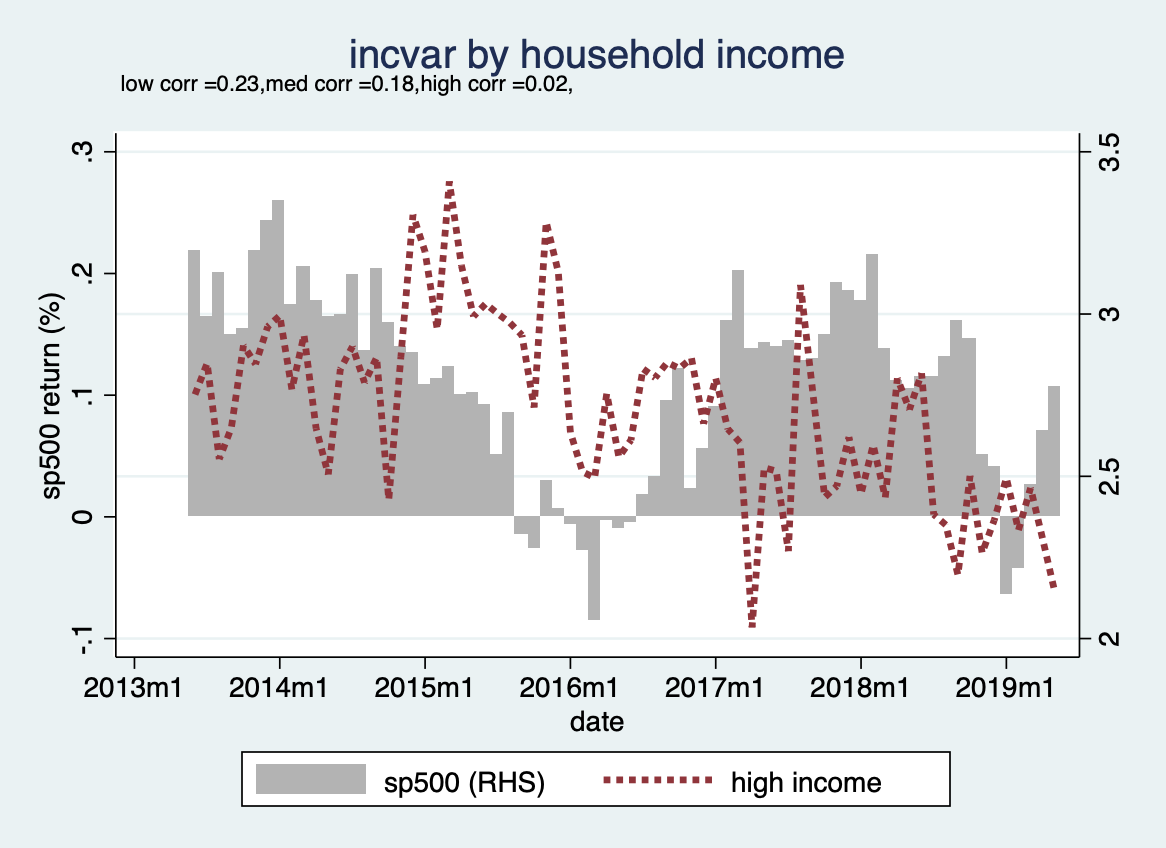
\includegraphics[width=0.8\textwidth, height=\0.4\textheight]{figures/ts_incvar_HHinc_g_mean_stk} \\
%		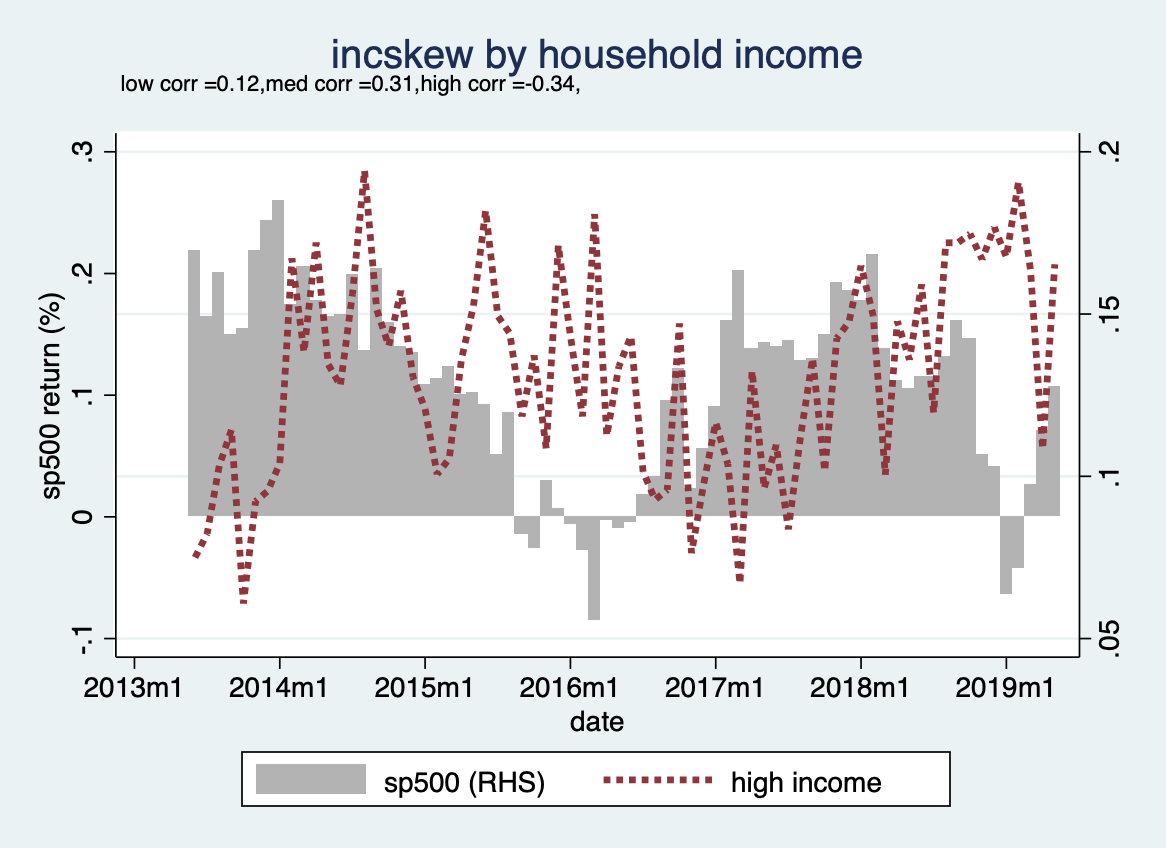
\includegraphics[width=0.8\textwidth, height=\0.4\textheight]{figures/ts_incskew_HHinc_g_mean_stk} 
%	\end{figure}
%\end{frame}



%\begin{frame}{Perceived correlaton with stock market by age}
%	\begin{figure}
%		\centering
%		\label{ts_stk_age_g}
%		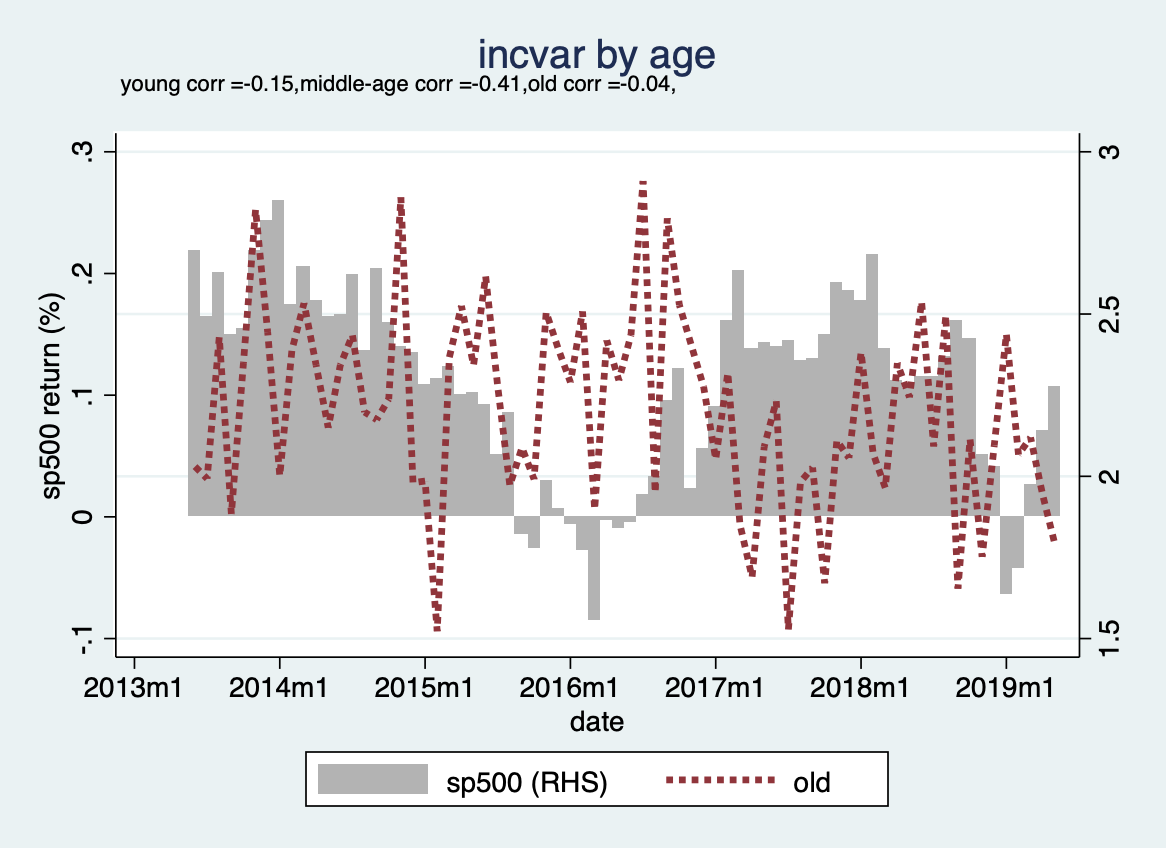
\includegraphics[width=0.8\textwidth, height=\0.4\textheight]{figures/ts_incvar_age_g_mean_stk} \\
%		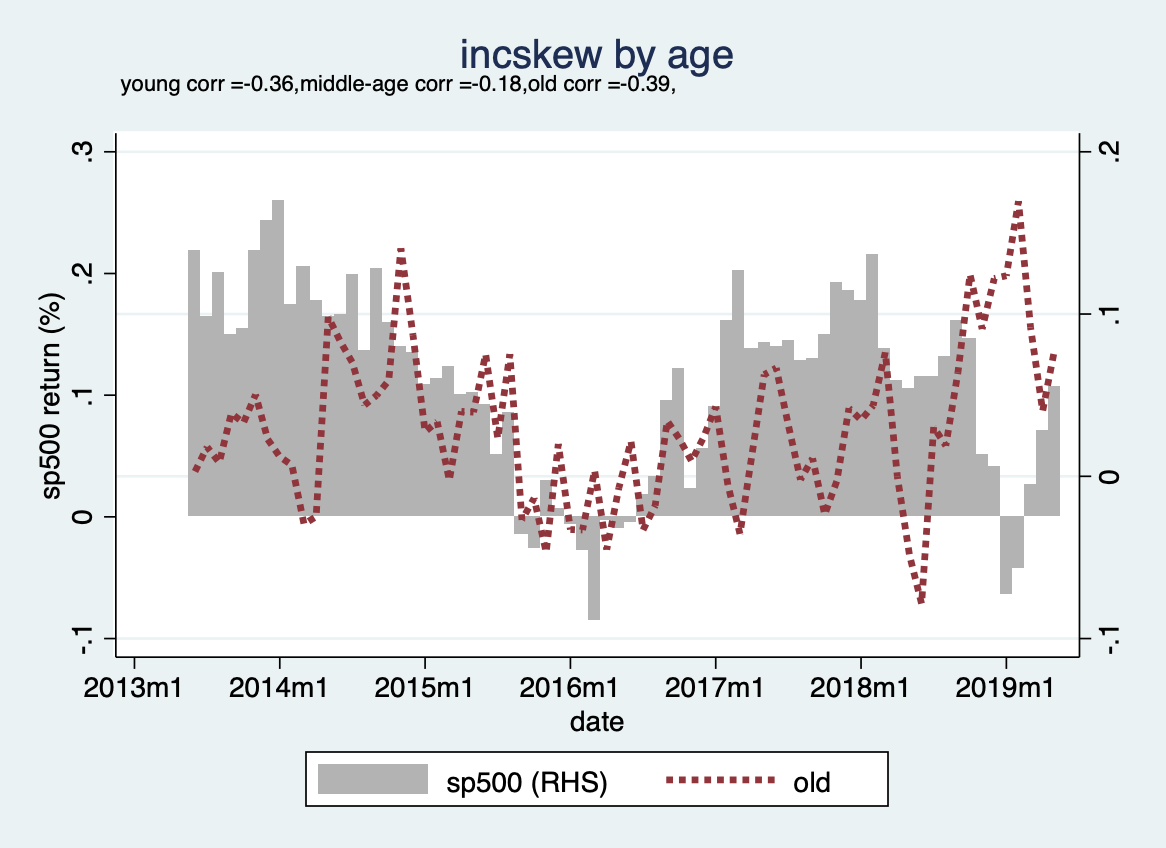
\includegraphics[width=0.8\textwidth, height=\0.4\textheight]{figures/ts_incskew_age_g_mean_stk} 
%	\end{figure}
%	\begin{itemize}
%		\item 
%	\end{itemize}
%\end{frame}



%\begin{frame}{Perceived correlaton with stock market by generation}
%	\begin{figure}
%		\centering
%		\label{ts_stk_byear_g}
%		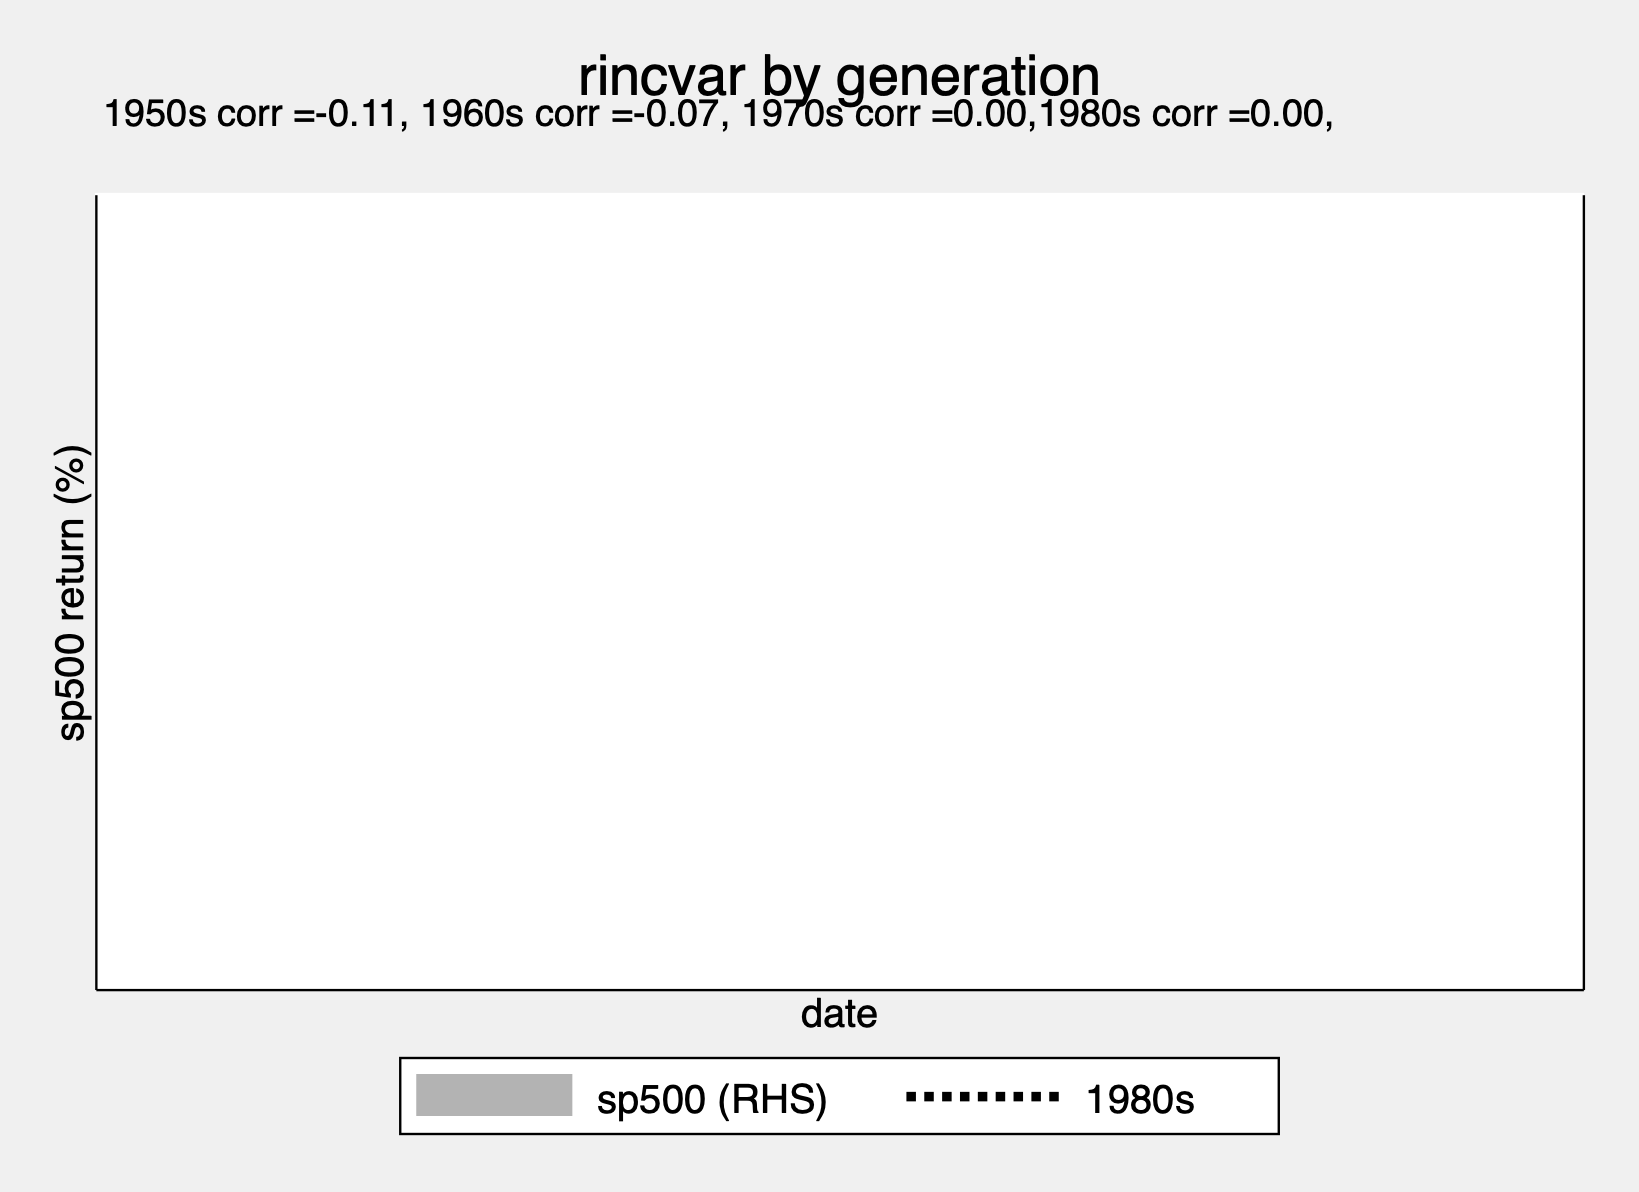
\includegraphics[width=0.8\textwidth, height=\0.4\textheight]{figures/ts_rincvar_byear_g_mean_stk} \\
%			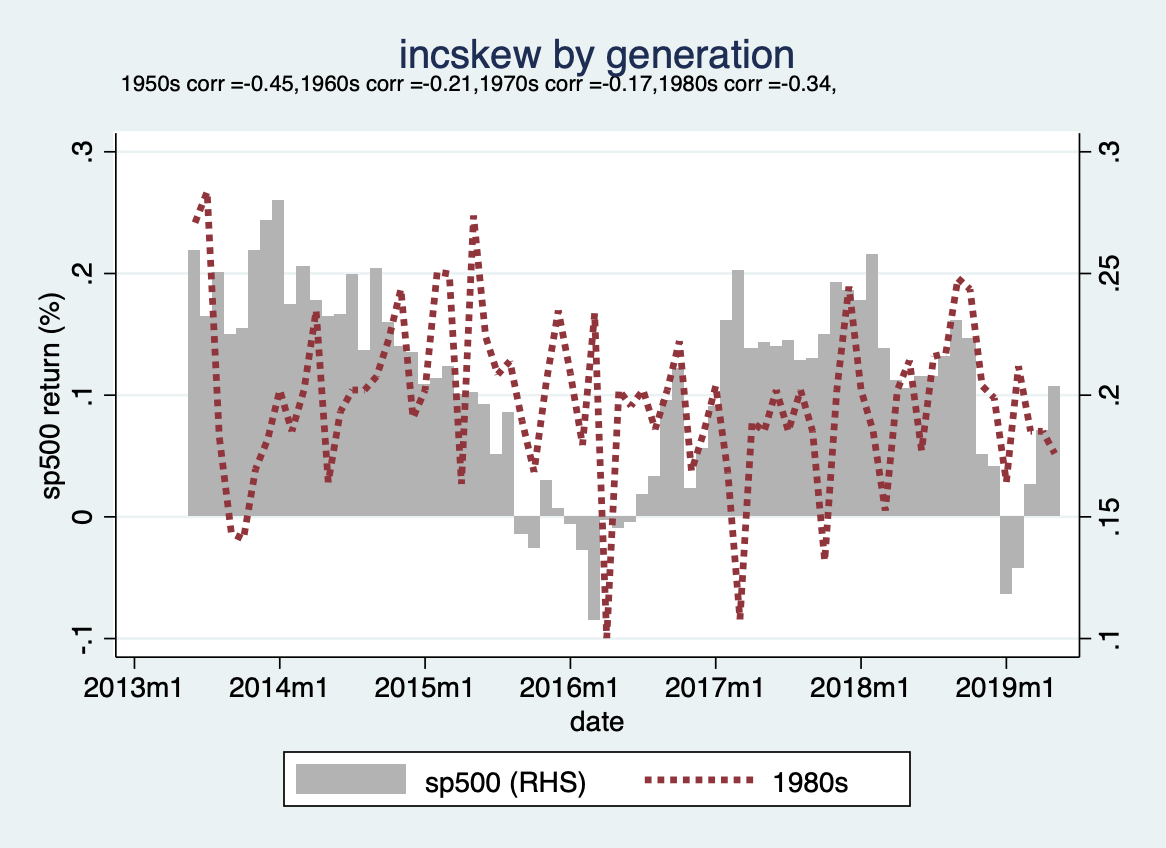
\includegraphics[width=0.8\textwidth, height=\0.4\textheight]{figures/ts_incskew_byear_g_median_stk} 
%	\end{figure}
%	\begin{itemize}
%		\item 
%	\end{itemize}
%\end{frame}


%\begin{frame}{Perceived correlaton with stock market by education}
%	\begin{figure}
%		\centering
%		\label{ts_stk_edu_g}
%		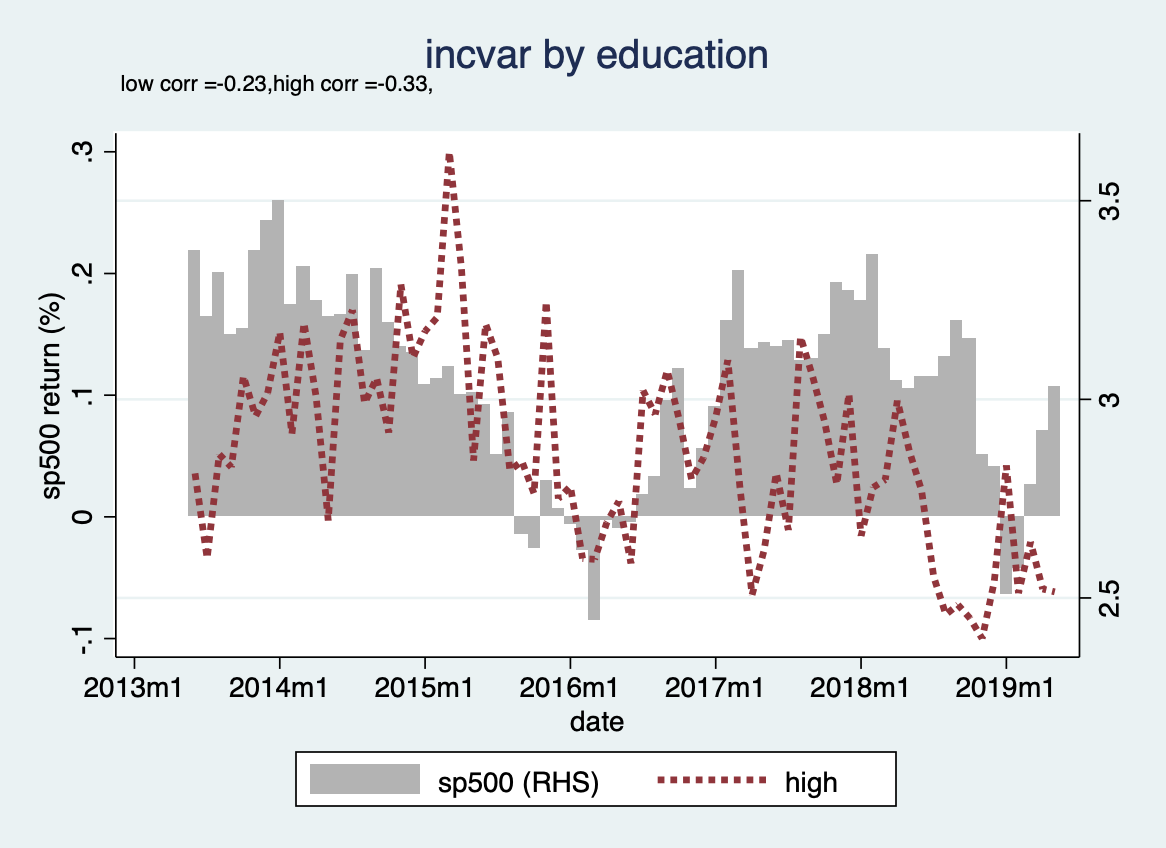
\includegraphics[width=0.8\textwidth, height=\0.4\textheight]{figures/ts_incvar_edu_g_mean_stk} \\
%			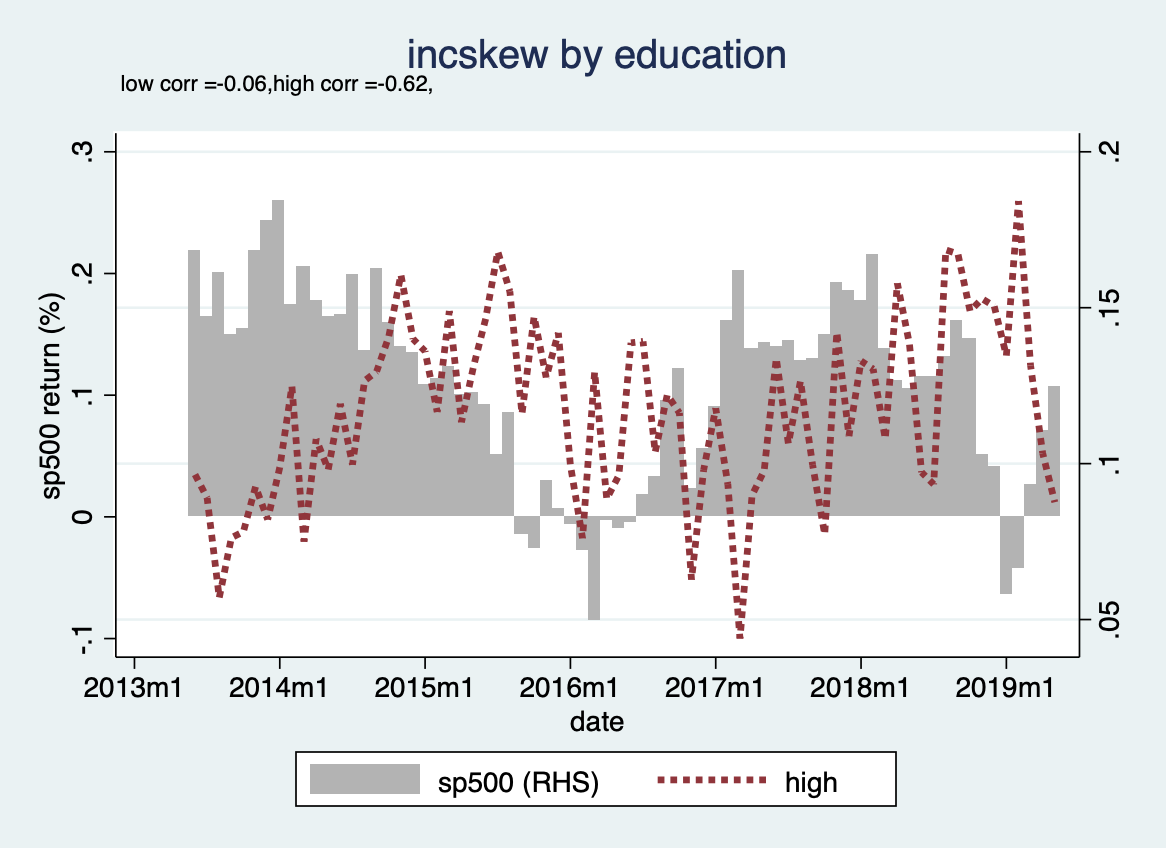
\includegraphics[width=0.8\textwidth, height=\0.4\textheight]{figures/ts_incskew_edu_g_mean_stk} 
%	\end{figure}
%	\begin{itemize}
%		\item 
%	\end{itemize}
%\end{frame}


\subsection{Permanent/transitory decomposition (work in progress)}

\begin{frame}{Underlying income process}
	
	\begin{itemize}
		\item Income of individual $i$, cohort $c$ at time $t$ 
		\begin{eqnarray*}
			\begin{split}
				& y_{i,c,t} = p_{i,c,t}+ \epsilon_{i,c,t},\quad \textrm{where } \epsilon_{i,c,t} \sim N(0,\sigma^2_{c,\epsilon}) \\
				& p_{i,c,t} = p_{i,c,t-1} + \theta_{i,c,t}, \quad \textrm{where }  \theta_{i,c,t} \sim N(0,\sigma^2_{\theta,c,t} ) \\
				& \log\sigma^2_{\theta,c,t} = \rho_c \log\sigma^2_{\theta,c,t-1} + \mu_{\theta,c,t}  \\
				& \mu_{\theta,c,t} \sim N(0,\gamma_c^2)
			\end{split}
		\end{eqnarray*}

	
		\item Parameters for cohort $c$
		\begin{itemize}
			\item $\rho_{c}$: how persistent is the innovation to the permanent risk  
			\item $\gamma_c$: how large is the innovation to the size of permanent risk
			\item $\sigma_{c,\epsilon}$: the time-invariant size of the transitory risk
		\end{itemize}
	\end{itemize}
\end{frame}


\begin{frame}{From monthly to yearly }
	\begin{itemize}
		\item Assuming the agent understands the process 
	\end{itemize}
	\begin{itemize}
		\item Perceived risks about \textcolor{blue}{next-month} growth $\Delta y_{i,t}$
		\begin{eqnarray*}
			\begin{split}
				& \overline {var_{i,t}}(\Delta y_{i,t+1}) & = E_{i,t}( {\sigma^2_{\theta,t+1}}) + \sigma^2_{\epsilon} \\
				& & = \rho e^{-0.5\gamma} \sigma^2_{i,\theta,t}  + \sigma^2_{\epsilon} 
			\end{split}
		\end{eqnarray*}
		
		\item Perceived risks about \textcolor{blue}{next-year} growth $\Delta Y_{i,t}$
		\begin{eqnarray*}
			\begin{split}
				& \overline {var_{i,t}}(\Delta Y_{i,t+12}) \\
				& = \sum^{12}_{k=1} (12-k)^2 E_{i,t}( {\sigma^2_{\theta,t+k}}) + 12^2 \sigma^2_{\epsilon} \\ 
				& = \sum^{12}_{k=1} (12-k)^2 \rho^k e^{-0.5k\gamma} \sigma^2_{i,\theta,t}+ 12^2 \sigma^2_{\epsilon}  	 
			\end{split}
		\end{eqnarray*}
	\end{itemize}
\end{frame}

%\begin{frame}{Perceived permanent and transitory decomposition}
%	\begin{enumerate}
%	\item SMM estimation using the following moments of perceptions 
%	\begin{itemize}
 %    \item average perceived risks, variance, autocovariance across the whole population or within specified cohort
%	\end{itemize}
%\item A breakdown of perceived risks into permanent and transitory components %With the estimated paramete, we will have a breakdown of the permanent and transitory risks. We can redo the exercises in previous sections seperately. 
%\end{enumerate}
%\end{frame}


\section{Model (work in progress)}

%\begin{frame}{Model ingredients}
	
%	\begin{enumerate}
%		\item imperfect understanding of the income process
		% a deviation from rational expectation benchmark. 
%		\begin{itemize}
%			\item past experiences $\rightarrow$ income risk perceptions
%		\end{itemize}
		%\item a life cycle with a constant probability of death 
		%\item uninsured idiosyncratic risks and aggregate risks %(the workhorse assumption of the HANK literature) 
		%\item single asset, i.e. no distinction between liquid and iliquid assets 
	%\end{enumerate}
%\end{frame}

%\begin{frame}{Intuitions behind the model mechanisms}
%	\begin{itemize}
%		\item an imperfect understanding $ \quad \rightarrow$ heterogeneous perception of risks $ \quad \text{AND } $ uninsurance of risks $ \quad \rightarrow$ difference in precautionary motives and MPCs across populations $ \quad \rightarrow$ potential amplification of aggregate MPC
%	\end{itemize}
%\end{frame}

%%%%%%%%%%%%%%%%%%%


%%%%%%%%%%%%%%%%%%%%%%%%%%%%%%%%%


\section*{Appendix}

\begin{frame}{Covariants of expected income growth}
	\begin{table}
		\centering
		\caption{Expected income growth and individual characteristics}
		\label{micro_reg_exp}
		\adjustbox{max height=0.5\textheight, max width=\textwidth}{ 
			\begin{tabular}{ccccccccc}
				\hline 
				{} &  incexp I & incexp II & incexp III & incexp IIII & rincexp I & rincexp II & rincexp III & rincexp IIII \\
				\hline 
				HHinc\_gr=low inc &           &           &      -0.03 &             &           &            &    -0.39*** &              \\
				&           &           &     (0.02) &             &           &            &      (0.03) &              \\
				educ\_gr=low educ &           &           &            &    -0.25*** &           &            &             &     -0.63*** \\
				&           &           &            &      (0.02) &           &            &             &       (0.03) \\
				gender=male      &           &           &            &    -0.32*** &           &            &             &     -0.78*** \\
				&           &           &            &      (0.02) &           &            &             &       (0.03) \\
				parttime=yes     &  -0.47*** &  -0.36*** &   -0.35*** &             &  -0.63*** &   -0.53*** &    -0.44*** &              \\
				&    (0.03) &    (0.03) &     (0.03) &             &    (0.04) &     (0.04) &      (0.04) &              \\
				selfemp=yes      &   0.86*** &  -0.00*** &    0.00*** &             &   0.84*** &   -0.00*** &    -0.00*** &              \\
				&    (0.03) &    (0.00) &     (0.00) &             &    (0.05) &     (0.00) &      (0.00) &              \\
				Stkprob          &           &   0.01*** &    0.01*** &             &           &    0.02*** &     0.02*** &              \\
				&           &    (0.00) &     (0.00) &             &           &     (0.00) &      (0.00) &              \\
				UEprobInd        &           &  -0.01*** &   -0.01*** &             &           &   -0.02*** &    -0.02*** &              \\
				&           &    (0.00) &     (0.00) &             &           &     (0.00) &      (0.00) &              \\
				Intercept        &   2.82*** &   2.57*** &    2.58*** &     3.05*** &  -0.29*** &   -0.92*** &    -0.80*** &      0.20*** \\
				&    (0.01) &    (0.02) &     (0.02) &      (0.02) &    (0.02) &     (0.03) &      (0.03) &       (0.02) \\
				\hline 
				N                &     54275 &     48606 &      48606 &       47712 &     49702 &      44446 &       44446 &        43694 \\
				R2               &      0.01 &      0.02 &       0.02 &        0.01 &      0.01 &       0.04 &        0.04 &         0.02 \\
				
				\hline 
			\end{tabular}
		}
	\end{table}
\end{frame}

\bibliographystyle{apalike}
\bibliography{PerceivedIncomeRisk}


\end{document}
